% Secure E2EE Chat Application - Project Report
% Information Security Semester Project
\documentclass[12pt,a4paper]{article}

% Packages
\usepackage[utf8]{inputenc}
\usepackage[margin=1.25in]{geometry}
\usepackage{graphicx}
\usepackage{amsmath}
\usepackage{amssymb}
\usepackage{algorithm}
\usepackage{algpseudocode}
\usepackage{listings}
\usepackage{xcolor}
\usepackage{tikz}
\usetikzlibrary{shapes,arrows,positioning,chains,fit,calc}
\usepackage{hyperref}
\usepackage{fancyhdr}
\usepackage{tcolorbox}
\usepackage{enumitem}
\usepackage{booktabs}
\usepackage{longtable}
\usepackage{multirow}
\usetikzlibrary{arrows.meta, positioning, calc, shapes, shadows, fit, backgrounds}
\usepackage{float}
\usepackage{caption}
\usepackage{xcolor}
\usepackage{titlesec}
\usepackage{soul}
\usepackage{geometry}
% Hyperref setup
\hypersetup{
    colorlinks=true,
    linkcolor=blue!80!black,
    filecolor=magenta,      
    urlcolor=blue!80!black,
    citecolor=blue!80!black,
    pdfauthor={Security Team},
    pdftitle={Secure E2EE Chat Application - Project Report},
    pdfsubject={Information Security Project},
}

% Professional color scheme
\definecolor{darkblue}{RGB}{26,59,108}
\definecolor{lightblue}{RGB}{65,105,225}
\definecolor{accentgreen}{RGB}{34,139,34}
\definecolor{darkgray}{RGB}{64,64,64}

% Custom box styling commands
\newcommand{\securitybox}[2]{%
\begin{tcolorbox}[
    colback=accentgreen!5,
    colframe=accentgreen!75!black,
    coltitle=white,
    colbacktitle=accentgreen!75!black,
    title=\textbf{#1},
    boxrule=1.5pt,
    arc=3pt,
    left=8pt,
    right=8pt,
    top=8pt,
    bottom=8pt
]
#2
\end{tcolorbox}%
}

\newcommand{\cryptobox}[2]{%
\begin{tcolorbox}[
    colback=lightblue!10,
    colframe=darkblue,
    coltitle=white,
    colbacktitle=darkblue,
    title=\textbf{#1},
    boxrule=1.5pt,
    arc=3pt,
    left=8pt,
    right=8pt,
    top=8pt,
    bottom=8pt
]
#2
\end{tcolorbox}%
}

\newcommand{\threatbox}[2]{%
\begin{tcolorbox}[
    colback=red!5,
    colframe=red!75!black,
    coltitle=white,
    colbacktitle=red!75!black,
    title=\textbf{#1},
    boxrule=1.5pt,
    arc=3pt,
    left=8pt,
    right=8pt,
    top=8pt,
    bottom=8pt
]
#2
\end{tcolorbox}%
}

% Code listing settings with professional styling
\lstset{
    basicstyle=\ttfamily\small,
    breaklines=true,
    frame=single,
    numbers=left,
    numberstyle=\tiny\color{darkgray},
    tabsize=2,
    captionpos=b,
    stringstyle=\color{red!70},
    commentstyle=\color{gray!70}\itshape,
    keywordstyle=\color{darkblue}\bfseries,
    backgroundcolor=\color{gray!5},
    rulecolor=\color{darkgray},
    framextopmargin=5pt,
    framexbottommargin=5pt
}

% Section and subsection styling
\titleformat{\section}
{\normalfont\Large\bfseries\color{darkblue}}
{\thesection}{1em}{\hrule\vspace{0.5em}}[\vspace{0.3em}]

\titleformat{\subsection}
{\normalfont\large\bfseries\color{darkblue}}
{\thesubsection}{0.8em}{}

\titleformat{\subsubsection}
{\normalfont\bfseries\color{lightblue}}
{\thesubsubsection}{0.6em}{}

% Header and footer with professional design
\pagestyle{fancy}
\fancyhf{}
\fancyhead[R]{\textcolor{darkblue}{\small\textbf{Secure E2EE Chat Application}}}
\fancyhead[L]{\textcolor{darkblue}{\small\textbf{Information Security}}}
\fancyfoot[C]{\thepage}
\renewcommand{\headrulewidth}{0.5pt}
\renewcommand{\headrule}{\color{lightblue}\hrule width\headwidth height\headrulewidth\kern-\headrulewidth}
\renewcommand{\footrulewidth}{0.5pt}
\renewcommand{\footrule}{\color{lightblue}\hrule width\headwidth height\footrulewidth\kern-\footrulewidth}

\begin{document}

% Title page with professional design
\begin{titlepage}
    \centering
    \color{darkblue}
    
    % Top border
    {\color{lightblue}\rule{\textwidth}{3pt}}
    
    \vspace{1.5cm}
    
    % --- University Name ---
    {\Large \textbf{NATIONAL UNIVERSITY OF COMPUTER AND EMERGING SCIENCES}}
    
    \vspace{0.8cm}
    
    % --- Logo ---
    \includegraphics[width=0.4\textwidth]{National_University_of_Computer_and_Emerging_Sciences_logo.png} 
    
    \vspace{1.5cm}
    
    % --- Course Name ---
    {\LARGE \textbf{INFORMATION SECURITY}}
    
    {\color{lightblue}\hrule \vspace{0.5cm}}
    
    % --- Project Title ---
    {\Huge \textbf{Secure End-to-End Encrypted\\Chat Application}}
    
    {\color{lightblue}\hrule \vspace{0.5cm}}
    
    % --- Semester Project ---
    {\Large \textit{Semester Project \quad | \quad Fall 2025}}
      
    \vfill
    
    % --- Group Members ---
    {\large \textbf{GROUP MEMBERS:}}
    
    \vspace{0.8cm}
    
    {\Large
    \begin{tabular}{l c r}
        \textbf{HASHIM AHMAD} & \quad & \textbf{22I-2478} \\[0.3cm]
        \textbf{SHOUKAT KHAN} & \quad & \textbf{22I-8784} \\[0.3cm]
        \textbf{MALAIKA REHMAN} & \quad & \textbf{22I-2605} \\
    \end{tabular}
    }
    
    \vspace{1.5cm}
    
    % --- Submission Date ---
    {\normalsize \textit{December 2025}}
    
    \vspace{1cm}
    
    % Bottom border
    {\color{lightblue}\rule{\textwidth}{3pt}}
     
\end{titlepage}
\thispagestyle{empty}
\newpage
% Table of Contents
{\color{darkblue}
\tableofcontents
}
\clearpage

% Abstract
\section*{Abstract}
\addcontentsline{toc}{section}{Abstract}

This report documents the design and implementation of a secure end-to-end encrypted (E2EE) chat application that demonstrates modern cryptographic principles and security best practices. The system employs industry-standard algorithms including RSA-PSS (2048-bit) for identity authentication, ECDH P-256 for ephemeral key agreement, and AES-256-GCM for authenticated encryption.

The architecture follows a zero-knowledge model where the server stores only ciphertext and never has access to decryption keys or plaintext communications. All cryptographic operations are performed client-side using the Web Crypto API, eliminating the need to trust the service provider. The implementation includes a three-layer replay protection mechanism combining timestamp validation, nonce deduplication, and sequence numbering to prevent message replay attacks.

The report includes comprehensive threat modeling using STRIDE analysis, detailed cryptographic protocol documentation, attack demonstrations illustrating both vulnerability and protection mechanisms, and evaluation of security properties. The system successfully implements confidentiality, integrity, authenticity, and non-repudiation guarantees suitable for sensitive communications.

\textbf{Keywords:} End-to-End Encryption, E2EE, Cryptography, Key Exchange Protocol, Web Crypto API, Zero-Knowledge Architecture, STRIDE Analysis, Replay Protection

\newpage

%==============================================================================
% SECTION 1: INTRODUCTION
%==============================================================================
\section{Introduction}
\label{sec:introduction}

\subsection{Overview}

In an era where digital privacy concerns are paramount, secure communication systems have become essential for protecting sensitive information from unauthorized access. This project implements a secure end-to-end encrypted (E2EE) chat application that demonstrates the practical application of modern cryptographic protocols and security principles in a web-based environment.

The application leverages the Web Crypto API (SubtleCrypto interface) to perform all cryptographic operations directly in the user's browser, ensuring that plaintext data never leaves the client device. This client-side encryption approach, combined with a zero-knowledge server architecture, provides strong security guarantees even if the server infrastructure is compromised.

\subsection{Motivation}

Traditional messaging applications often rely on server-side encryption, where the service provider has access to decryption keys and can potentially access user communications. This centralized trust model creates several security and privacy concerns:

\begin{itemize}
    \item \textbf{Server Compromise}: If the server is breached, all user communications are exposed
    \item \textbf{Legal Compulsion}: Service providers may be legally required to provide access to user data
    \item \textbf{Insider Threats}: System administrators have potential access to sensitive communications
    \item \textbf{Data Retention}: Servers storing plaintext create long-term security liabilities
\end{itemize}

End-to-end encryption addresses these concerns by ensuring that only the communicating parties can decrypt messages, eliminating the need to trust the service provider with sensitive data.

\subsection{Project Objectives}

The primary objectives of this project are:

\begin{enumerate}
    \item \textbf{Implement Secure Cryptographic Protocols}: Utilize industry-standard algorithms (RSA-PSS, ECDH, AES-GCM) through the Web Crypto API
    \item \textbf{Zero-Knowledge Architecture}: Design a system where the server acts purely as a mailbox, never accessing plaintext data
    \item \textbf{Attack Resistance}: Implement protections against common attacks including MITM, replay, and eavesdropping
    \item \textbf{Demonstrate Security Properties}: Provide practical demonstrations of both secure and insecure implementations
    \item \textbf{Comprehensive Auditing}: Log security-relevant events for analysis and forensics
    \item \textbf{User Experience}: Balance strong security with usability
\end{enumerate}

%==============================================================================
% SECTION 2: PROBLEM STATEMENT
%==============================================================================
\section{Problem Statement and Requirements}
\label{sec:problem}

\subsection{Problem Definition}

The fundamental problem addressed by this project is:

\begin{tcolorbox}[
    colback=lightblue!10,
    colframe=darkblue,
    coltitle=white,
    colbacktitle=darkblue,
    title=\textbf{Core Problem},
    boxrule=2pt,
    arc=4pt,
    left=10pt,
    right=10pt,
    top=10pt,
    bottom=10pt
]
Design and implement a secure communication system where two parties can exchange messages and files with cryptographic guarantees of confidentiality, integrity, and authenticity, while minimizing trust requirements in the communication infrastructure.
\end{tcolorbox}

\subsection{Security Requirements}

\securitybox{Key Security Requirements}{
\textbf{Confidentiality (C):} Messages and files must be encrypted end-to-end; server must not access plaintext.\\
\textbf{Integrity (I):} Detect any tampering with messages, metadata, or file contents.\\
\textbf{Authenticity (A):} Verify sender identity and detect unauthorized key exchanges.\\
\textbf{Operational (O):} Provide cryptographic proofs of security events and maintain comprehensive audit logs.
}

\subsubsection{Confidentiality Requirements}

\begin{enumerate}[label=\textbf{C\arabic*:}]
    \item Messages must be encrypted end-to-end; the server cannot read plaintext
    \item Private cryptographic keys must never leave the client device in plaintext
    \item Session keys must be derived securely and known only to communicating parties
    \item File contents must be encrypted before upload to the server
    \item Encrypted data must use authenticated encryption to prevent tampering
\end{enumerate}

\subsubsection{Integrity Requirements}

\begin{enumerate}[label=\textbf{I\arabic*:}]
    \item Messages must be protected against modification in transit
    \item Digital signatures must authenticate the source of key exchange messages
    \item Authenticated encryption must detect any tampering with ciphertext
    \item Replay attacks must be detected and prevented
    \item Message ordering must be verifiable
\end{enumerate}

\subsubsection{Authenticity Requirements}

\begin{enumerate}[label=\textbf{A\arabic*:}]
    \item Users must prove identity using cryptographic credentials
    \item Key exchange messages must be digitally signed
    \item Each message must be verifiably from the claimed sender
    \item Man-in-the-middle attacks must be prevented through signature verification
\end{enumerate}

\subsubsection{Availability and Operational Requirements}

\begin{enumerate}[label=\textbf{O\arabic*:}]
    \item The system must gracefully handle network failures
    \item Session state must be recoverable after client restart
    \item Audit logs must track security-relevant events
    \item Error messages must not leak sensitive information
    \item Memory containing cryptographic material must be properly cleaned
\end{enumerate}
\newpage
%==============================================================================
% SECTION 3: THREAT MODEL (STRIDE)
%==============================================================================
\section{Threat Modeling (STRIDE Analysis)}
\label{sec:threat-model}

\subsection{Overview}

This section analyzes potential threats to the secure E2EE chat application using the STRIDE methodology. STRIDE categorizes security threats into six classes: Spoofing, Tampering, Repudiation, Information Disclosure, Denial of Service, and Elevation of Privilege. For each threat category, we identify specific threats relevant to this system, describe their potential impact, and explain how the implemented security mechanisms mitigate them.

\subsection{Spoofing Threats}

\subsubsection{S1: Identity Spoofing}

\textbf{Threat Description}: An attacker attempts to impersonate another user by falsely claiming their identity or obtaining their public key.

\textbf{Impact}: Attacker could establish fraudulent sessions and intercept communications.

\textbf{Mitigation}:
\begin{itemize}
    \item Unique usernames enforced at registration
    \item RSA-PSS digital signatures bind identity keys to usernames
    \item Private keys never leave the client, preventing key theft
\end{itemize}

\subsubsection{S2: Key Exchange Man-in-the-Middle (MITM)}

\textbf{Threat Description}: An attacker intercepts the key exchange and substitutes their own ephemeral ECDH public keys, positioning themselves between two legitimate users.

\textbf{Impact}: Complete loss of message confidentiality and integrity; attacker can read and modify all communications.

\textbf{Mitigation}:
\begin{itemize}
    \item ECDH ephemeral public keys are digitally signed using identity private keys (RSA-PSS or ECDSA)
    \item Signature verification using the peer's published public key prevents key substitution
    \item Failed signature verification aborts key exchange and triggers \texttt{MITM\_ATTACK\_DETECTED} audit event
    \item Demo implementation (Section \ref{sec:mitm-demo}) shows both vulnerable and protected scenarios
\end{itemize}

\subsubsection{S3: Session Hijacking}

\textbf{Threat Description}: Attacker attempts to take over an established session by injecting forged messages or stealing session keys.

\textbf{Impact}: Unauthorized message transmission, impersonation of legitimate users.

\textbf{Mitigation}:
\begin{itemize}
    \item Session keys derived from authenticated ECDH exchange
    \item Every message includes sequence numbers and nonces
    \item Out-of-order or duplicate messages rejected by server
    \item Session key stored only in memory (client) and cleared on logout
\end{itemize}

\subsection{Tampering Threats}

\subsubsection{T1: Message Tampering}

\textbf{Threat Description}: Attacker modifies encrypted messages in transit or while stored on the server.

\textbf{Impact}: Undetected message corruption, potential command injection in deserialized payloads.

\textbf{Mitigation}:
\begin{itemize}
    \item AES-256-GCM provides authenticated encryption with 128-bit authentication tag
    \item Any modification to ciphertext causes authentication failure and message rejection
    \item Integrity violations logged as security events
\end{itemize}

\subsubsection{T2: Key Exchange Message Manipulation}

\textbf{Threat Description}: Attacker modifies ephemeral ECDH public keys or digital signatures during transmission.

\textbf{Impact}: Forged signatures could enable MITM attacks if verification is bypassed.

\textbf{Mitigation}:
\begin{itemize}
    \item All key exchange messages digitally signed
    \item Signature verification detects any bit-level modifications
    \item Failed verification immediately aborts key exchange
\end{itemize}

\subsubsection{T3: Replay Protection Bypass}

\textbf{Threat Description}: Attacker attempts to manipulate or forge nonces, timestamps, or sequence numbers to bypass replay protection.

\textbf{Impact}: Successful replays could duplicate messages or execute commands multiple times.

\textbf{Mitigation}:
\begin{itemize}
    \item Metadata (sequence, timestamp, nonce) authenticated by GCM tag
    \item Server-side validation prevents acceptance of altered metadata
    \item Three independent replay checks (timestamp, nonce deduplication, sequence ordering) provide defense-in-depth
    \item Demo implementation shows successful blocking of multiple replay scenarios
\end{itemize}

\subsection{Repudiation Threats}

\subsubsection{R1: Message Origin Denial}

\textbf{Threat Description}: User denies sending a message or claims a message was forged.

\textbf{Impact}: Loss of accountability in communications.

\textbf{Mitigation}:
\begin{itemize}
    \item All key exchange messages digitally signed with timestamps
    \item Message metadata (sender, sequence, timestamp) included in encrypted payload
    \item Comprehensive audit logs record all security events
    \item Limitations: Full non-repudiation would require timestamp authority and long-term archival of signatures
\end{itemize}

\subsubsection{R2: Audit Log Tampering}

\textbf{Threat Description}: User or attacker attempts to delete or modify audit logs to hide malicious activity.

\textbf{Impact}: Loss of evidence for security investigation.

\textbf{Mitigation}:
\begin{itemize}
    \item Audit logs stored server-side in MongoDB
    \item Users cannot modify logs (read-only access)
    \item Timestamps from trusted server clock
    \item API access controls restrict log access
\end{itemize}

\subsection{Information Disclosure Threats}

\subsubsection{ID1: Server Compromise - Data Breach}

\textbf{Threat Description}: Attacker gains complete access to server database and attempts to extract plaintext messages or encryption keys.

\textbf{Impact}: Without E2EE, this would compromise all user communications.

\textbf{Mitigation}:
\begin{itemize}
    \item \textbf{Zero-Knowledge Architecture}: Server stores only ciphertext; no plaintext messages exist on server
    \item Private keys never transmitted to server; stored encrypted client-side
    \item Session keys derived client-side only; server never has access
    \item Per-file encryption keys wrapped with session keys
    \item \textbf{Result}: Server compromise does not expose plaintext or session keys
\end{itemize}

\subsubsection{ID2: Network Eavesdropping}

\textbf{Threat Description}: Passive attacker monitors network traffic to intercept encrypted messages.

\textbf{Impact}: Attacker captures ciphertext but cannot decrypt without session key.

\textbf{Mitigation}:
\begin{itemize}
    \item HTTPS/TLS encrypts data in transit
    \item Even if HTTPS is compromised, E2EE provides additional encryption layer
    \item Message payloads encrypted end-to-end before HTTPS transmission
    \item Double encryption: application-level (E2EE) + transport-level (TLS)
\end{itemize}

\subsubsection{ID3: Client-Side Storage Compromise}

\textbf{Threat Description}: Attacker gains access to browser's IndexedDB and attempts to extract stored private keys.

\textbf{Impact}: Private key theft could enable impersonation and message decryption.

\textbf{Mitigation}:
\begin{itemize}
    \item Private keys encrypted with PBKDF2-derived keys before storage
    \item PBKDF2 with 150,000 iterations (200-400ms per key derivation) resists brute-force attacks
    \item Attacker needs both: (1) IndexedDB access AND (2) user's password
    \item Single factor compromise (IndexedDB only) insufficient for key theft
\end{itemize}

\subsubsection{ID4: Memory Extraction}

\textbf{Threat Description}: Attacker with system-level access (malware, rootkit) extracts cryptographic keys from process memory.

\textbf{Impact}: Session keys or private keys in memory could be stolen.

\textbf{Mitigation}:
\begin{itemize}
    \item Session keys cleared on logout and session reset
    \item ECDH ephemeral keys cleared after session key derivation
    \item Sensitive data overwritten where possible
    \item Limitations: Complete protection requires OS-level secure memory (beyond project scope)
\end{itemize}

\subsection{Denial of Service Threats}

\subsubsection{DoS1: Message Flooding}

\textbf{Threat Description}: Attacker floods the server with large numbers of encrypted messages to exhaust computational resources.

\textbf{Impact}: Server becomes unresponsive; legitimate users cannot communicate.

\textbf{Mitigation}:
\begin{itemize}
    \item Input validation on all API endpoints
    \item Early rejection of malformed messages (fail-fast design)
    \item Replay protection checks fail quickly (timestamp before decryption)
    \item Server-side rate limiting (production implementation detail)
\end{itemize}

\subsubsection{DoS2: Key Exchange Disruption}

\textbf{Threat Description}: Attacker interferes with key exchange by sending invalid requests or responses.

\textbf{Impact}: Users cannot establish sessions; communication disabled.

\textbf{Mitigation}:
\begin{itemize}
    \item Signature verification fails for invalid key exchange messages
    \item Failed exchanges are logged and reported to users
    \item Users can retry key exchange
    \item Timeout mechanisms prevent stalled exchanges from consuming resources
\end{itemize}

\subsubsection{DoS3: Storage Exhaustion}

\textbf{Threat Description}: Attacker uploads large files or generates excessive log entries to exhaust disk space.

\textbf{Impact}: Server runs out of storage; service becomes unavailable.

\textbf{Mitigation}:
\begin{itemize}
    \item File size limits enforced on upload
    \item Automatic cleanup of old nonces (older than 30 seconds)
    \item Audit log retention policies (production consideration)
\end{itemize}

\subsection{Elevation of Privilege Threats}

\subsubsection{EoP1: Unauthorized Message Access}

\textbf{Threat Description}: User attempts to read messages intended for other users.

\textbf{Impact}: Breach of message confidentiality between other users.

\textbf{Mitigation}:
\begin{itemize}
    \item Messages encrypted with session keys derived from authenticated key exchange between two parties only
    \item Only the two communicating parties can derive the session key
    \item Cannot decrypt without possessing the correct session key
    \item Server-side access controls verify recipient before returning messages
\end{itemize}

\subsubsection{EoP2: Cryptographic Downgrade Attack}

\textbf{Threat Description}: Attacker attempts to force use of weaker cryptographic algorithms (e.g., downgrade from RSA-2048 to smaller key sizes).

\textbf{Impact}: Reduced cryptographic strength; vulnerability to brute-force attacks.

\textbf{Mitigation}:
\begin{itemize}
    \item No algorithm negotiation; algorithms are hardcoded
    \item RSA-2048-bit minimum (no smaller sizes supported)
    \item AES-256-GCM only (no fallback to AES-128 or CBC mode)
    \item ECDH P-256 only (no weaker curves)
    \item Web Crypto API enforces correct algorithm implementation
\end{itemize}

\subsubsection{EoP3: Signature Verification Bypass}

\textbf{Threat Description}: Attacker attempts to forge signatures or exploit signature verification logic.

\textbf{Impact}: Key exchange MITM attack succeeds; attacker gains message decryption capability.

\textbf{Mitigation}:
\begin{itemize}
    \item Signature verification using Web Crypto API (standard-compliant implementation)
    \item Failed verification throws exception; no partial acceptance
    \item Signature check mandatory before accepting any key exchange public key
    \item No alternative or legacy verification logic
\end{itemize}

\subsection{Threat Summary Matrix}

\begin{table}[H]
\centering
\small
\begin{tabular}{@{}llcc@{}}
\toprule
\textbf{Threat Category} & \textbf{Specific Threat} & \textbf{Likelihood} & \textbf{Mitigation} \\ \midrule
\multirow{3}{*}{Spoofing} & Identity spoofing & Low & Digital signatures \\
 & MITM attack & Low & Signature verification \\
 & Session hijacking & Low & Sequence + nonce checks \\
\midrule
\multirow{3}{*}{Tampering} & Message tampering & Low & AES-GCM tag \\
 & Key exchange tampering & Low & Digital signatures \\
 & Replay bypass & Very Low & Triple-layer protection \\
\midrule
\multirow{2}{*}{Repudiation} & Origin denial & Medium & Audit logs \\
 & Log tampering & Low & Server-side storage \\
\midrule
\multirow{4}{*}{Info Disclosure} & Server breach & Very Low & Zero-knowledge arch. \\
 & Network eavesdropping & Low & E2EE + TLS \\
 & Client storage breach & Medium & PBKDF2 encryption \\
 & Memory extraction & Medium & Key cleanup \\
\midrule
\multirow{3}{*}{Denial of Service} & Message flooding & Medium & Input validation \\
 & Key exchange disruption & Low & Signature checks \\
 & Storage exhaustion & Low & Size limits \\
\midrule
\multirow{3}{*}{Elevation of Privilege} & Unauthorized message access & Very Low & Session key isolation \\
 & Cryptographic downgrade & Very Low & No negotiation \\
 & Signature bypass & Very Low & Web Crypto API \\
\bottomrule
\end{tabular}
\caption{Threat Summary Matrix (Likelihood: Very Low = Infeasible, Low = Unlikely, Medium = Possible)}
\label{tab:threat-matrix}
\end{table}

\newpage
%==============================================================================
% SECTION 4: CRYPTOGRAPHIC DESIGN
%==============================================================================
\section{Cryptographic Design}
\label{sec:crypto}

\subsection{Overview}

The application implements a rigorous cryptographic architecture using industry-standard algorithms from the Web Crypto API. The design organizes cryptography into four domains:

\begin{enumerate}
    \item \textbf{Identity Management}: RSA-PSS (2048-bit) for user authentication and digital signatures
    \item \textbf{Key Exchange}: ECDH P-256 ephemeral keys with signature authentication for session establishment
    \item \textbf{Data Encryption}: AES-256-GCM for authenticated encryption of all messages and files
    \item \textbf{Key Derivation}: PBKDF2 for password-to-key conversion and HKDF for shared-secret-to-session-key derivation
\end{enumerate}

\subsection{Cryptographic Primitives}

\subsubsection{RSA-PSS: Identity Key Signatures}

RSA-PSS with 2048-bit keys provides user identity authentication. The 2048-bit modulus offers 112 bits of equivalent symmetric security, meeting NIST baseline recommendations through 2030. Each user generates one RSA key pair during registration: the private key is encrypted with a password-derived key and stored locally, while the public key is sent to the server for signature verification during key exchange.

The algorithm uses SHA-256 hashing and full-length salt (32 bytes) to prevent signature recovery attacks. The probabilistic nature ensures that signing the same message twice produces different signatures, enhancing security against pattern analysis.

\subsubsection{ECDH P-256: Ephemeral Key Agreement}

Elliptic Curve Diffie-Hellman over the NIST P-256 curve enables ephemeral key agreement. Each key exchange generates fresh P-256 key pairs that are used once and then discarded, providing forward secrecy: compromise of long-term identity keys does not reveal past session keys because ephemeral keys were never stored.

The P-256 curve (secp256r1) provides 128 bits of equivalent security and is the most widely supported ECC curve in Web Crypto API. The shared secret produced by ECDH is 32 bytes (256 bits), providing sufficient entropy for session key derivation.

\subsubsection{AES-256-GCM: Authenticated Encryption}

AES-256-GCM combines AES encryption with Galois Counter Mode authentication, providing both confidentiality and integrity in a single operation. The algorithm uses:

\begin{itemize}
    \item \textbf{256-bit key}: Maximum AES key size
    \item \textbf{96-bit IV (nonce)}: Recommended GCM nonce size; prevents collisions
    \item \textbf{128-bit authentication tag}: Detects any tampering with ciphertext or metadata
\end{itemize}

Each message uses a unique, randomly-generated 96-bit IV. This uniqueness is critical: reusing an IV under the same key breaks GCM security by enabling keystream recovery and authentication tag forgery. The 128-bit tag provides 128 bits of authentication strength, making tag forgery computationally infeasible.

\subsubsection{PBKDF2-HMAC-SHA-256: Password-Based Key Derivation}

PBKDF2 converts user passwords into 256-bit keys for encrypting long-term private keys stored in IndexedDB. The algorithm mitigates password guessing attacks through computational cost: each password candidate requires 150,000 HMAC-SHA-256 iterations.

\begin{itemize}
    \item \textbf{150,000 iterations}: Provides strong offline brute-force resistance while maintaining acceptable login latency (200-400ms)
    \item \textbf{32-byte salt}: Prevents rainbow table attacks; each user has a unique salt
    \item \textbf{Trade-off}: Strong passwords are essential; weak passwords can still be cracked offline despite the iteration count
\end{itemize}

\subsubsection{HKDF-SHA-256: Key Derivation from Shared Secrets}

HKDF (HMAC-based Key Derivation Function) converts ECDH shared secrets into session encryption keys. The algorithm follows the RFC 5869 extract-then-expand paradigm:

\begin{itemize}
    \item \textbf{Extract}: HMAC-SHA-256 produces a pseudorandom key from the ECDH shared secret
    \item \textbf{Expand}: Additional HMAC operations stretch the key and derive the final session key with domain separation (info="E2EE\_SESSION\_KEY")
\end{itemize}

Domain separation prevents key confusion: different info strings produce independent keys even from the same shared secret. This protects against key derivation attacks.

\subsection{Critical Security Invariants}

The cryptographic design enforces six non-negotiable security requirements:

\securitybox{Security Invariants}{
\textbf{1. Nonce Uniqueness:} Each message uses distinct 96-bit IV (violation → keystream recovery)\\[4pt]
\textbf{2. Private Key Storage:} Long-term keys encrypted with PBKDF2 before IndexedDB storage\\[4pt]
\textbf{3. Signature Verification:} All ECDH ephemeral keys verified with peer's RSA key (omission → MITM)\\[4pt]
\textbf{4. Session Key Isolation:} Unique session key per conversation, never reused\\[4pt]
\textbf{5. Timestamp Tolerance:} Messages within ±30 seconds of server time (prevents long-duration replays)\\[4pt]
\textbf{6. Server Key Isolation:} Server stores no plaintext keys, passwords, or private data
}                                                   

\subsection{Cryptographic Strength Summary}

\begin{table}[H]
\centering
\small
\begin{tabular}{@{}lll@{}}
\toprule
\textbf{Algorithm} & \textbf{Configuration} & \textbf{Equivalent Security} \\ \midrule
RSA-PSS & 2048-bit, SHA-256 & 112 bits \\
ECDH & P-256 & 128 bits \\
AES-256-GCM & 256-bit key, 96-bit IV & 256-bit (encryption), 128-bit (auth) \\
PBKDF2 & 150k iterations & Strong (password-dependent) \\
HKDF & SHA-256 & 256 bits \\
\bottomrule
\end{tabular}
\caption{Cryptographic Strength Comparison}
\label{tab:crypto-strength}
\end{table}

\cryptobox{Security Strength Analysis}{
\textbf{Minimum Security Level:} RSA-PSS (112 bits), acceptable because:\\
\hspace*{0.5cm}• Identity keys are long-lived, used infrequently\\
\hspace*{0.5cm}• Forward secrecy via ephemeral ECDH keys (128 bits)\\
\hspace*{0.5cm}• NIST allows 2048-bit RSA until 2030\\[6pt]
\textbf{Strongest Elements:} AES-256-GCM (256-bit) for message encryption and session key wrapping.
}


\section{Key Exchange Protocol Diagrams}

\subsection{Complete Key Exchange Flow}
\begin{figure}[H]
\centering
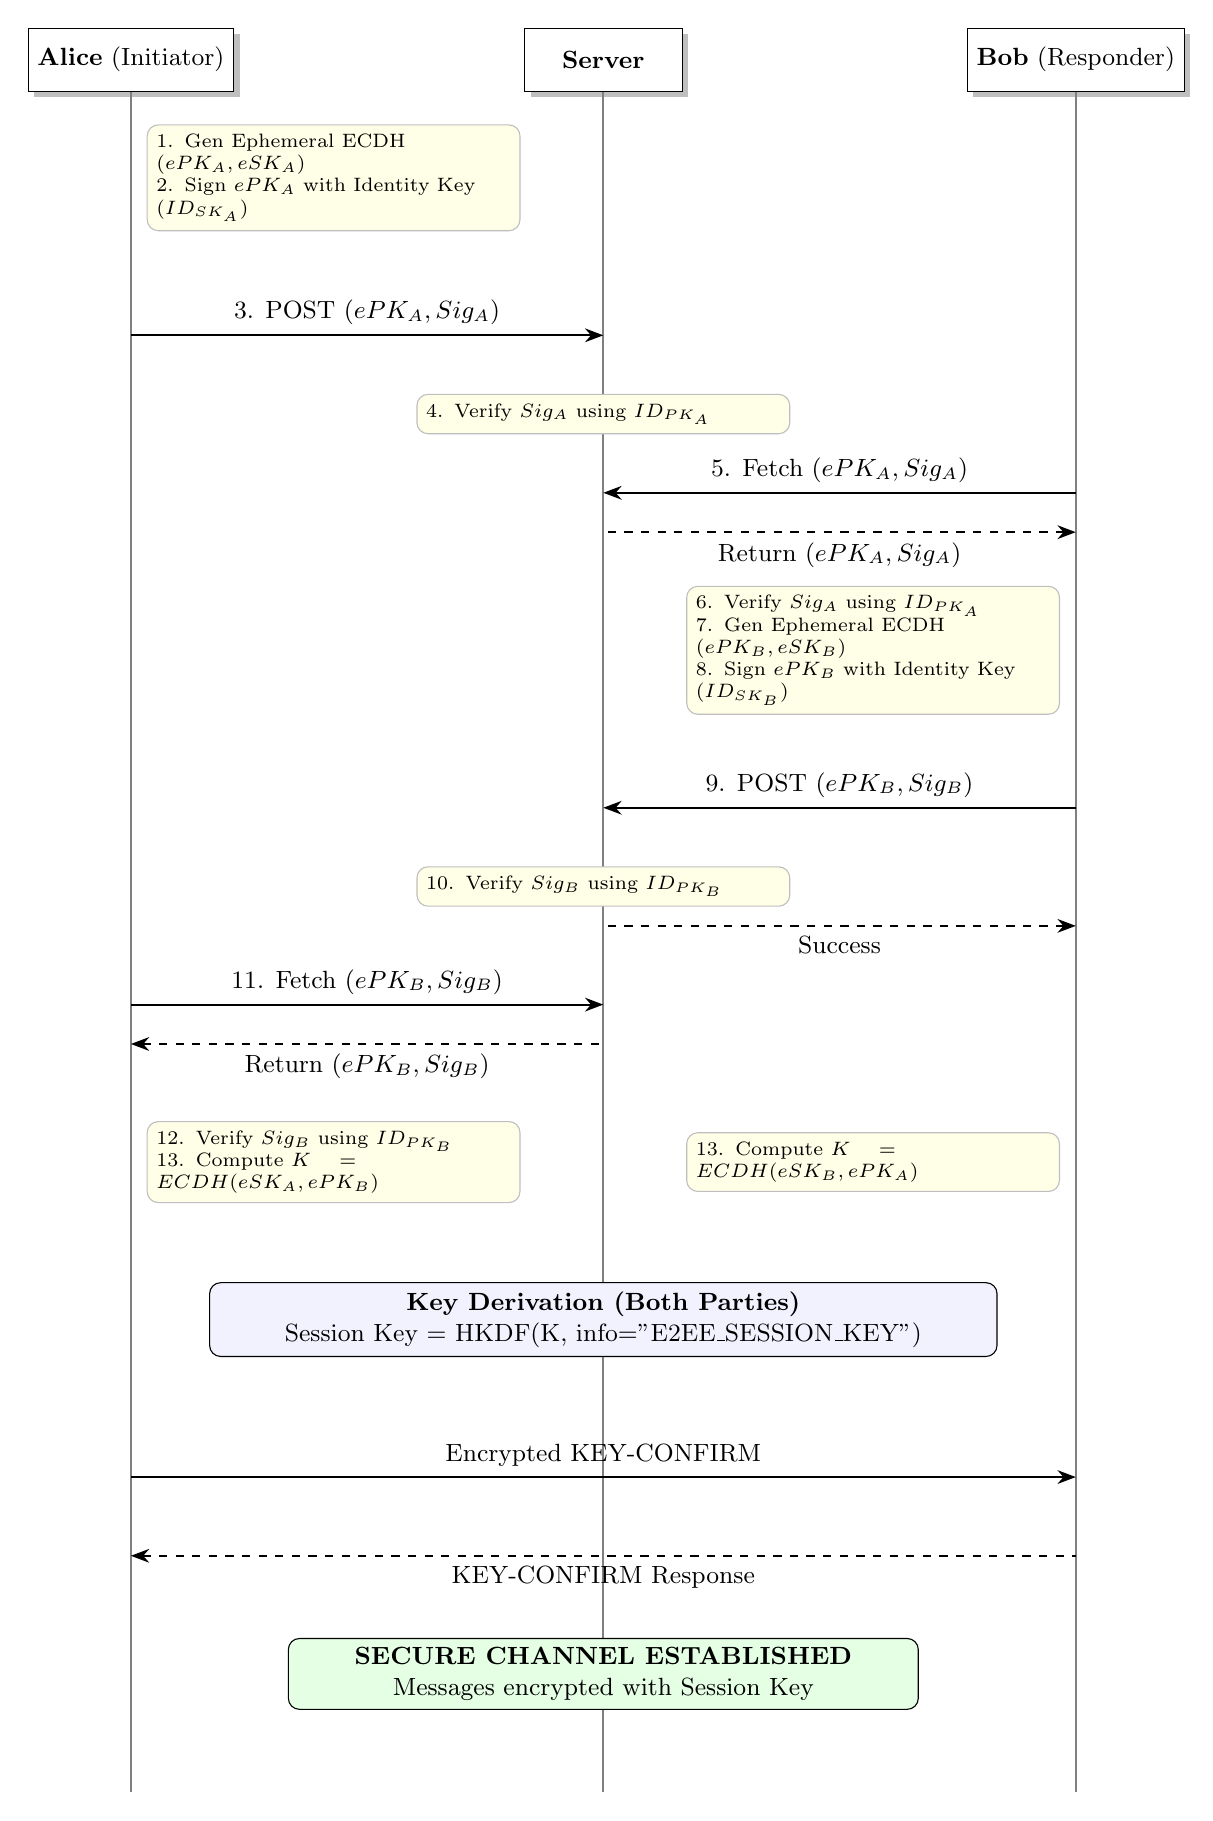
\begin{tikzpicture}[
    >=Stealth, 
    node distance=1.5cm, 
    font=\small,
    actor/.style={draw, rectangle, minimum width=2cm, minimum height=0.8cm, fill=white, drop shadow},
    lifeline/.style={draw=gray, thick},
    msg/.style={->, thick},
    return/.style={<-, dashed, thick},
    note/.style={draw=gray!50, fill=yellow!10, rectangle, rounded corners, align=left, font=\scriptsize, text width=4.5cm, anchor=west}
]

    % --- Actors ---
    \node[actor] (Alice) at (0,0) {\textbf{Alice} (Initiator)};
    \node[actor] (Server) at (6,0) {\textbf{Server}};
    \node[actor] (Bob) at (12,0) {\textbf{Bob} (Responder)};

    % --- Lifelines ---
    \draw[lifeline] (Alice) -- (0,-22);
    \draw[lifeline] (Server) -- (6,-22);
    \draw[lifeline] (Bob) -- (12,-22);

    % --- Step 1: Alice Setup ---
    \node[note] at (0.2, -1.5) {
        1. Gen Ephemeral ECDH ($ePK_A, eSK_A$)\\
        2. Sign $ePK_A$ with Identity Key ($ID_{SK_A}$)
    };

    % --- Step 2: Upload to Server ---
    \draw[msg] (0,-3.5) -- node[midway, above] {3. POST ($ePK_A, Sig_A$)} (6,-3.5);

    % --- Server Verification ---
    \node[note, anchor=center] at (6, -4.5) {
        4. Verify $Sig_A$ using $ID_{PK_A}$
    };

    % --- Step 3: Bob Fetch ---
    \draw[msg] (12,-5.5) -- node[midway, above] {5. Fetch ($ePK_A, Sig_A$)} (6,-5.5);
    \draw[return] (12,-6.0) -- node[midway, below] {Return ($ePK_A, Sig_A$)} (6,-6.0);

    % --- Step 4: Bob Processing ---
    \node[note, anchor=east] at (11.8, -7.5) {
        6. Verify $Sig_A$ using $ID_{PK_A}$\\
        7. Gen Ephemeral ECDH ($ePK_B, eSK_B$)\\
        8. Sign $ePK_B$ with Identity Key ($ID_{SK_B}$)
    };

    % --- Step 5: Bob Upload ---
    \draw[msg] (12,-9.5) -- node[midway, above] {9. POST ($ePK_B, Sig_B$)} (6,-9.5);
    
    % --- Server Verification ---
    \node[note, anchor=center] at (6, -10.5) {
        10. Verify $Sig_B$ using $ID_{PK_B}$
    };
    
    \draw[return] (12,-11.0) -- node[midway, below] {Success} (6,-11.0);

    % --- Step 6: Alice Fetch ---
    \draw[msg] (0,-12.0) -- node[midway, above] {11. Fetch ($ePK_B, Sig_B$)} (6,-12.0);
    \draw[return] (0,-12.5) -- node[midway, below] {Return ($ePK_B, Sig_B$)} (6,-12.5);

    % --- Step 7: Final Computation (Alice) ---
    \node[note] at (0.2, -14.0) {
        12. Verify $Sig_B$ using $ID_{PK_B}$\\
        13. Compute $K = ECDH(eSK_A, ePK_B)$
    };

    % --- Step 7: Final Computation (Bob) ---
    \node[note, anchor=east] at (11.8, -14.0) {
        13. Compute $K = ECDH(eSK_B, ePK_A)$
    };

    % --- Derivation ---
    \node[draw, fill=blue!5, rectangle, rounded corners, align=center, minimum width=10cm] at (6, -16) {
        \textbf{Key Derivation (Both Parties)}\\
        Session Key = HKDF(K, info="E2EE\_SESSION\_KEY")
    };

    % --- Key Confirmation ---
    \draw[msg] (0,-18) -- node[midway, above] {Encrypted KEY-CONFIRM} (12,-18);
    \draw[return] (0,-19) -- node[midway, below] {KEY-CONFIRM Response} (12,-19);
    
    % --- Secure Channel Established ---
    \node[draw, fill=green!10, rectangle, rounded corners, align=center, minimum width=8cm] at (6, -20.5) {
        \textbf{SECURE CHANNEL ESTABLISHED}\\
        Messages encrypted with Session Key
    };

\end{tikzpicture}
\end{figure}

\subsection{Replay Protection Validation}

\begin{figure}[H]
\centering
\begin{tikzpicture}[
    node distance=1cm,
    check/.style={rectangle, draw, minimum width=5cm, minimum height=1cm, align=center, fill=orange!20},
    pass/.style={rectangle, draw, minimum width=3cm, minimum height=0.7cm, align=center, fill=green!30},
    fail/.style={rectangle, draw, minimum width=3cm, minimum height=0.7cm, align=center, fill=red!30},
    arrow/.style={->, >=stealth, thick}
]

\node[check] (msg) {Incoming Encrypted Message};

% Nonce check
\node[check, below=1.5cm of msg] (nonce) {Check 1: Nonce Uniqueness\\Query conversation.recentNonces};
\node[pass, below left=0.8cm and 2cm of nonce] (nonce-pass) {✓ Nonce Unique};
\node[fail, below right=0.8cm and 2cm of nonce] (nonce-fail) {✗ Duplicate Nonce\\REPLAY BLOCKED};

\draw[arrow] (msg) -- (nonce);
\draw[arrow] (nonce) -| (nonce-pass);
\draw[arrow] (nonce) -| (nonce-fail);

% Timestamp check
\node[check, below=2cm of nonce] (time) {Check 2: Timestamp\\$|now - timestamp| < 30s$};
\node[pass, below left=0.8cm and 2cm of time] (time-pass) {✓ Within Window};
\node[fail, below right=0.8cm and 2cm of time] (time-fail) {✗ Outside Window\\REPLAY BLOCKED};

\draw[arrow] (nonce-pass) |- (time);
\draw[arrow] (time) -| (time-pass);
\draw[arrow] (time) -| (time-fail);

% Sequence check
\node[check, below=2cm of time] (seq) {Check 3: Sequence Number\\$seq > lastSequence$};
\node[pass, below left=0.8cm and 2cm of seq] (seq-pass) {✓ Increasing};
\node[fail, below right=0.8cm and 2cm of seq] (seq-fail) {✗ Non-increasing\\REPLAY BLOCKED};

\draw[arrow] (time-pass) |- (seq);
\draw[arrow] (seq) -| (seq-pass);
\draw[arrow] (seq) -| (seq-fail);

% Final
\node[pass, below=1.5cm of seq, minimum width=6cm, minimum height=1cm] (accept) {\Large ✓ Message Accepted\\Store and Deliver};

\draw[arrow] (seq-pass) |- (accept);

\end{tikzpicture}
\end{figure}
\newpage

\section{Encryption/Decryption Workflows}
\label{sec:encryption-decryption}

This section describes how messages and files are encrypted and decrypted in the application. All encryption uses AES-256-GCM, an authenticated encryption algorithm that protects both confidentiality and integrity.

\subsection{Message Encryption Workflow}

\subsubsection{Overview}

When a user sends a message, the application encrypts it client-side using the session key established during key exchange. The server receives and stores only the ciphertext, never accessing plaintext.

\subsubsection{Encryption Process}

The message encryption process involves the following steps:

\begin{enumerate}
    \item \textbf{Metadata Generation}: The sender generates four cryptographic values:
    \begin{itemize}
        \item A 128-bit random nonce (unique identifier per message for replay detection)
        \item A 96-bit random IV (initialization vector for AES-GCM)
        \item Current timestamp in milliseconds
        \item Sequence number (counter incremented per message sent in the conversation)
    \end{itemize}
    
    \item \textbf{Payload Construction}: A JSON object is created containing the plaintext message, sender username, and all metadata values. This object is encoded to UTF-8 bytes.
    
    \item \textbf{AES-256-GCM Encryption}: The AES-GCM algorithm encrypts the payload using:
    \begin{itemize}
        \item The 256-bit session key from key exchange
        \item The 96-bit random IV
        \item Additional Authenticated Data: \texttt{sender|sequence|timestamp} (authenticated but not encrypted)
    \end{itemize}
    
    \item \textbf{Tag Inclusion}: AES-GCM produces a ciphertext with a 128-bit authentication tag automatically appended. This tag proves no tampering occurred.
    
    \item \textbf{Base64 Encoding}: All binary values (ciphertext with tag, IV, nonce) are Base64-encoded for JSON transmission.
    
    \item \textbf{HTTPS Transmission and Server Storage}: The encrypted message packet is sent to the server via HTTPS POST. The server receives and stores the ciphertext with associated metadata (sender, receiver, sequence, timestamp, nonce) in the Message database, but never decrypts it.
\end{enumerate}

\subsubsection{Encryption Workflow Diagram}

\begin{figure}[H]
\centering
\begin{tikzpicture}[
    node distance=1.2cm,
    process/.style={rectangle, draw, minimum width=5cm, minimum height=0.8cm, align=center, fill=blue!10, rounded corners},
    input/.style={rectangle, draw, minimum width=5cm, minimum height=0.8cm, align=center, fill=cyan!20, rounded corners},
    output/.style={rectangle, draw, minimum width=5cm, minimum height=0.8cm, align=center, fill=green!20, rounded corners},
    crypto/.style={rectangle, draw=thick, minimum width=5cm, minimum height=0.9cm, align=center, fill=orange!20, rounded corners},
    arrow/.style={->, >=stealth, thick}
]

    % Input
    \node[input] (plaintext) at (5, 10) {Plaintext Message};
    
    % Step 1: Generate metadata
    \node[process] (metadata) at (5, 8.8) {Generate Sequence, Nonce\\Timestamp};
    \draw[arrow] (plaintext) -- (metadata);
    
    % Step 2: Create payload
    \node[process] (payload) at (5, 7.6) {Create JSON Payload\\with Metadata};
    \draw[arrow] (metadata) -- (payload);
    
    % Step 3: Encode
    \node[process] (encode) at (5, 6.4) {Encode to UTF-8 Bytes};
    \draw[arrow] (payload) -- (encode);
    
    % Step 4: Generate cryptographic values
    \node[process] (geniv) at (2, 5.2) {Generate 96-bit IV\\(CSPRNG)};
    \draw[arrow] (encode) |- (geniv);
    
    \node[input] (sessionkey) at (8, 5.2) {Session Key\\(32 bytes from HKDF)};
    
    % Step 5: Encrypt
    \node[crypto] (encrypt) at (5, 3.8) {AES-256-GCM Encrypt\\(plaintext, key, iv)};
    \draw[arrow] (geniv) -- (encrypt);
    \draw[arrow] (sessionkey) -- (encrypt);
    
    % Step 6: Extract components
    \node[process] (extract) at (2, 2.6) {Extract Ciphertext};
    \node[process] (tag) at (8, 2.6) {Extract Auth Tag\\(128 bits)};
    \draw[arrow] (encrypt) |- (extract);
    \draw[arrow] (encrypt) |- (tag);
    
    % Step 7: Encode for transmission
    \node[process] (transmit) at (5, 1.4) {Encode to Base64\\for HTTP};
    \draw[arrow] (extract) -- (transmit);
    \draw[arrow] (tag) -- (transmit);
    
    % Output
    \node[output] (encrypted) at (5, 0.2) {Encrypted Message Packet};
    \draw[arrow] (transmit) -- (encrypted);

\end{tikzpicture}
\caption{Message Encryption Workflow}
\label{fig:encrypt-workflow}
\end{figure}

\subsection{Message Decryption Workflow}

\subsubsection{Overview}

When the receiver is online, the client fetches encrypted messages from the server. Before decryption, the application validates replay protection mechanisms to prevent attackers from wasting CPU resources with invalid messages.

\subsubsection{Decryption Process}

The decryption process follows these steps:

\begin{enumerate}
    \item \textbf{Component Extraction}: The received message contains the Base64-encoded ciphertext, IV, and plaintext metadata (sender, sequence, timestamp, nonce). All Base64 values are decoded to binary format.
    
    \item \textbf{Timestamp Validation (Layer 1)}: The server checks that the message timestamp falls within ±30 seconds of current server time. Messages older than 30 seconds or more than 30 seconds in the future are rejected immediately. This prevents long-duration replay attacks while accommodating reasonable network latency and clock skew.
    
    \item \textbf{Nonce Uniqueness Check (Layer 2)}: The server maintains a list of seen nonces per conversation. If the nonce has been received before, the message is rejected as a replay. Old nonces (beyond 30 seconds) are automatically removed from the list to prevent unbounded growth.
    
    \item \textbf{Sequence Number Validation (Layer 3)}: The server tracks the last sequence number received from each sender per conversation. If the message's sequence number does not exceed the last recorded sequence, the message is rejected. This ensures messages are accepted in order and prevents duplicate delivery.
    
    \item \textbf{AES-256-GCM Decryption}: After all replay checks pass, the ciphertext is decrypted using AES-GCM with:
    \begin{itemize}
        \item The session key (known only to the intended recipient)
        \item The extracted IV
        \item The same Additional Authenticated Data from encryption
    \end{itemize}
    During decryption, GCM verifies the authentication tag. If the tag does not match (indicating tampering or wrong key), decryption fails with an exception and no plaintext is revealed.
    
    \item \textbf{Payload Parsing}: The decrypted payload is parsed as JSON to extract the message content, sender, and metadata. The sender username is verified against the outer message metadata for consistency.
    
    \item \textbf{Display and Logging}: The message is displayed to the user with sender information and timestamp. A security event is logged recording the successful decryption.
\end{enumerate}

\subsubsection{Three-Layer Replay Protection Design}

The decryption process implements three independent layers of replay protection:

\begin{itemize}
    \item \textbf{Timestamp Layer}: Prevents replays beyond 30 seconds (the network communication window)
    \item \textbf{Nonce Layer}: Prevents duplication within the 30-second window using collision-resistant 128-bit random values
    \item \textbf{Sequence Layer}: Ensures strict ordering and prevents out-of-order message acceptance
\end{itemize}

An attacker must defeat all three layers simultaneously to successfully replay a message, making replay attacks infeasible.

\begin{enumerate}
    \item \textbf{UTF-8 Decoding}: Converts the decrypted bytes back to a UTF-8 string
    \item \textbf{JSON Parsing}: Parses the JSON to extract the message object containing sender username, message text, and redundant metadata
    \item \textbf{Integrity Verification}: Compares the sender username in the decrypted payload against the sender in the outer metadata. If they disagree, the message is rejected as corrupted or tampered
\end{enumerate}

\subsubsection{Decryption Process: Step 7 - Message Delivery to User Interface}

The receiver's application displays the message to the user with the following information:

\begin{itemize}
    \item \textbf{Sender}: The verified sender username
    \item \textbf{Message Text}: The plaintext message content
    \item \textbf{Timestamp}: The delivery time (when received), optionally compared to the message creation timestamp
    \item \textbf{Security Status}: Visual indicator that the message is encrypted and authenticated
    \item \textbf{Security Event Logging}: A security event is logged recording successful decryption, sender, sequence number, and timestamp
\end{itemize}

\subsubsection{Decryption Workflow Diagram}


\begin{figure}[H]
\centering
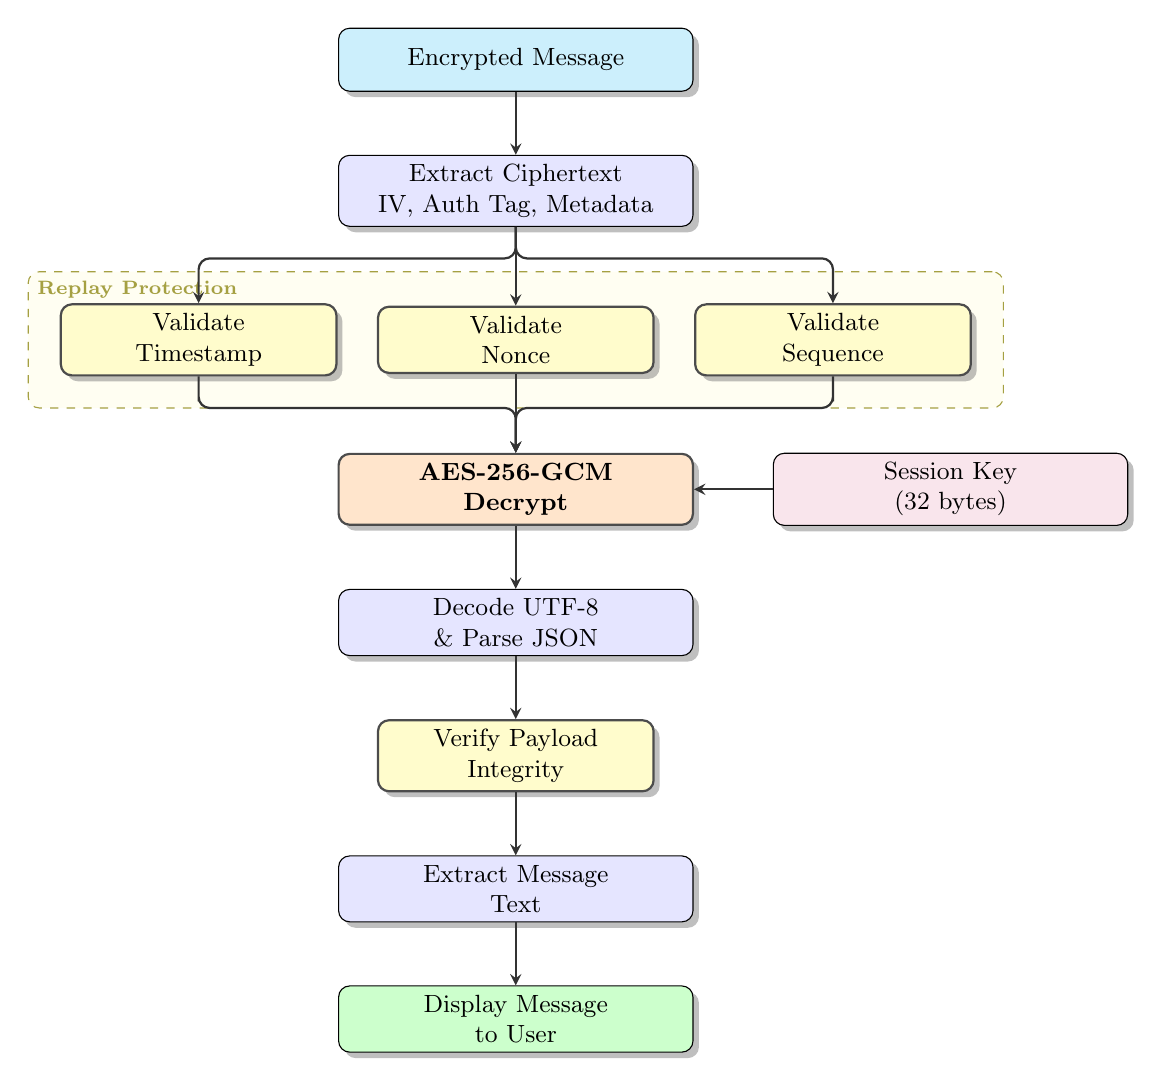
\begin{tikzpicture}[
    node distance=0.8cm and 0.5cm,
    process/.style={rectangle, draw, minimum width=4.5cm, minimum height=0.8cm, align=center, fill=blue!10, rounded corners, drop shadow, font=\small},
    input/.style={rectangle, draw, minimum width=4.5cm, minimum height=0.8cm, align=center, fill=cyan!20, rounded corners, drop shadow, font=\small},
    output/.style={rectangle, draw, minimum width=4.5cm, minimum height=0.8cm, align=center, fill=green!20, rounded corners, drop shadow, font=\small},
    crypto/.style={rectangle, draw=black!70, thick, minimum width=4.5cm, minimum height=0.9cm, align=center, fill=orange!20, rounded corners, drop shadow, font=\small\bfseries},
    validation/.style={rectangle, draw=black!70, thick, minimum width=3.5cm, minimum height=0.8cm, align=center, fill=yellow!20, rounded corners, drop shadow, font=\small},
    arrow/.style={->, >=stealth, thick, rounded corners, color=black!80}
]

    % --- Main Flow Column ---
    
    % Input
    \node[input] (encrypted) {Encrypted Message};
    
    % Step 1
    \node[process, below=of encrypted] (extract) {Extract Ciphertext\\IV, Auth Tag, Metadata};
    
    % Step 2-4: Parallel Validations
    % Centered validation node
    \node[validation, below=1cm of extract] (val-nonce) {Validate\\Nonce};
    % Left and Right validation nodes
    \node[validation, left=0.5cm of val-nonce] (val-ts) {Validate\\Timestamp};
    \node[validation, right=0.5cm of val-nonce] (val-seq) {Validate\\Sequence};
    
    % Step 5: Decrypt
    \node[crypto, below=1cm of val-nonce] (decrypt) {AES-256-GCM\\Decrypt};
    
    % Session Key Input (Side)
    \node[input, right=1cm of decrypt, fill=purple!10] (sessionkey) {Session Key\\(32 bytes)};
    
    % Step 6: Decode
    \node[process, below=of decrypt] (decode) {Decode UTF-8\\\& Parse JSON};
    
    % Step 7: Verify Payload
    \node[validation, below=of decode] (verify) {Verify Payload\\Integrity};
    
    % Step 8: Extract Message
    \node[process, below=of verify] (extract-msg) {Extract Message\\Text};
    
    % Step 9: Output
    \node[output, below=of extract-msg] (display) {Display Message\\to User};

    % --- Connections ---
    
    \draw[arrow] (encrypted) -- (extract);
    
    % Fork to validations
    \draw[arrow] (extract.south) -- ++(0,-0.4) -| (val-ts.north);
    \draw[arrow] (extract.south) -- (val-nonce.north);
    \draw[arrow] (extract.south) -- ++(0,-0.4) -| (val-seq.north);
    
    % Merge to decrypt
    \draw[arrow] (val-ts.south) |- ++(0,-0.4) -| (decrypt.north);
    \draw[arrow] (val-nonce.south) -- (decrypt.north);
    \draw[arrow] (val-seq.south) |- ++(0,-0.4) -| (decrypt.north);
    
    % Session Key input
    \draw[arrow] (sessionkey) -- (decrypt);
    
    % Linear flow downwards
    \draw[arrow] (decrypt) -- (decode);
    \draw[arrow] (decode) -- (verify);
    \draw[arrow] (verify) -- (extract-msg);
    \draw[arrow] (extract-msg) -- (display);

    % --- Background Grouping ---
    \begin{scope}[on background layer]
        \node[draw=yellow!60!black, dashed, fill=yellow!5, fit=(val-ts) (val-seq) (val-nonce), inner sep=0.4cm, rounded corners, label={[anchor=north west, font=\scriptsize\bfseries, text=yellow!60!black]north west:Replay Protection}] {};
    \end{scope}

\end{tikzpicture}
\caption{Message Decryption Workflow with Replay Protection}
\label{fig:decrypt-workflow}
\end{figure}

\subsection{File Encryption and Decryption}

\subsubsection{Overview: Double Encryption Architecture}

File encryption uses double encryption with key isolation:

\begin{enumerate}
    \item \textbf{Layer 1}: Each file is encrypted with a unique 256-bit key using AES-256-GCM
    \item \textbf{Layer 2}: The file encryption key is itself encrypted with the session key (also AES-256-GCM)
    \item \textbf{Result}: Key isolation—compromising one file key does not affect other files or the session key
\end{enumerate}

\subsubsection{File Encryption Process}

\begin{enumerate}
    \item \textbf{File Selection}: User selects file from filesystem. Client reads complete file into memory as binary data.
    
    \item \textbf{Per-File Key Generation}: A unique 256-bit random key and 96-bit random IV are generated using the CSPRNG. Each file uses a distinct key, even within the same conversation.
    
    \item \textbf{File Encryption}: File content is encrypted with AES-256-GCM using the per-file key. The 128-bit authentication tag is automatically appended by GCM.
    
    \item \textbf{Key Wrapping}: The per-file key is encrypted (wrapped) with the session key using AES-256-GCM with a separate IV. This creates a 48-byte wrapped key (32 bytes encrypted key + 16-byte tag).
    
    \item \textbf{Packet Assembly}: Client constructs upload packet containing:
    \begin{itemize}
        \item Encrypted file (Base64)
        \item File IV (Base64)
        \item Wrapped file key (Base64)
        \item Key wrap IV (Base64)
        \item Plaintext metadata: sender, receiver, filename, MIME type, file size
    \end{itemize}
    
    \item \textbf{Upload}: Packet is transmitted via HTTPS POST. Server stores in FileMessage database without accessing encrypted content.
\end{enumerate}

\subsubsection{File Decryption Process}

\begin{enumerate}
    \item \textbf{Packet Retrieval}: Receiver fetches encrypted file packet from server and decodes all Base64 components.
    
    \item \textbf{Key Unwrapping}: Wrapped file key is decrypted using the session key. AES-GCM automatically verifies the authentication tag. If verification fails, the key is corrupted or tampered.
    
    \item \textbf{File Decryption}: Decrypted per-file key is used to decrypt the file using AES-256-GCM. Authentication tag is verified. Decryption fails if tampering is detected.
    
    \item \textbf{File Reconstruction}: Decrypted bytes are wrapped in a Blob object with the correct MIME type. A download URL is created and triggered, allowing the user to save the file.
\end{enumerate}

\subsubsection{File Encryption and Decryption Workflow Diagram}

\begin{figure}[H]
\centering
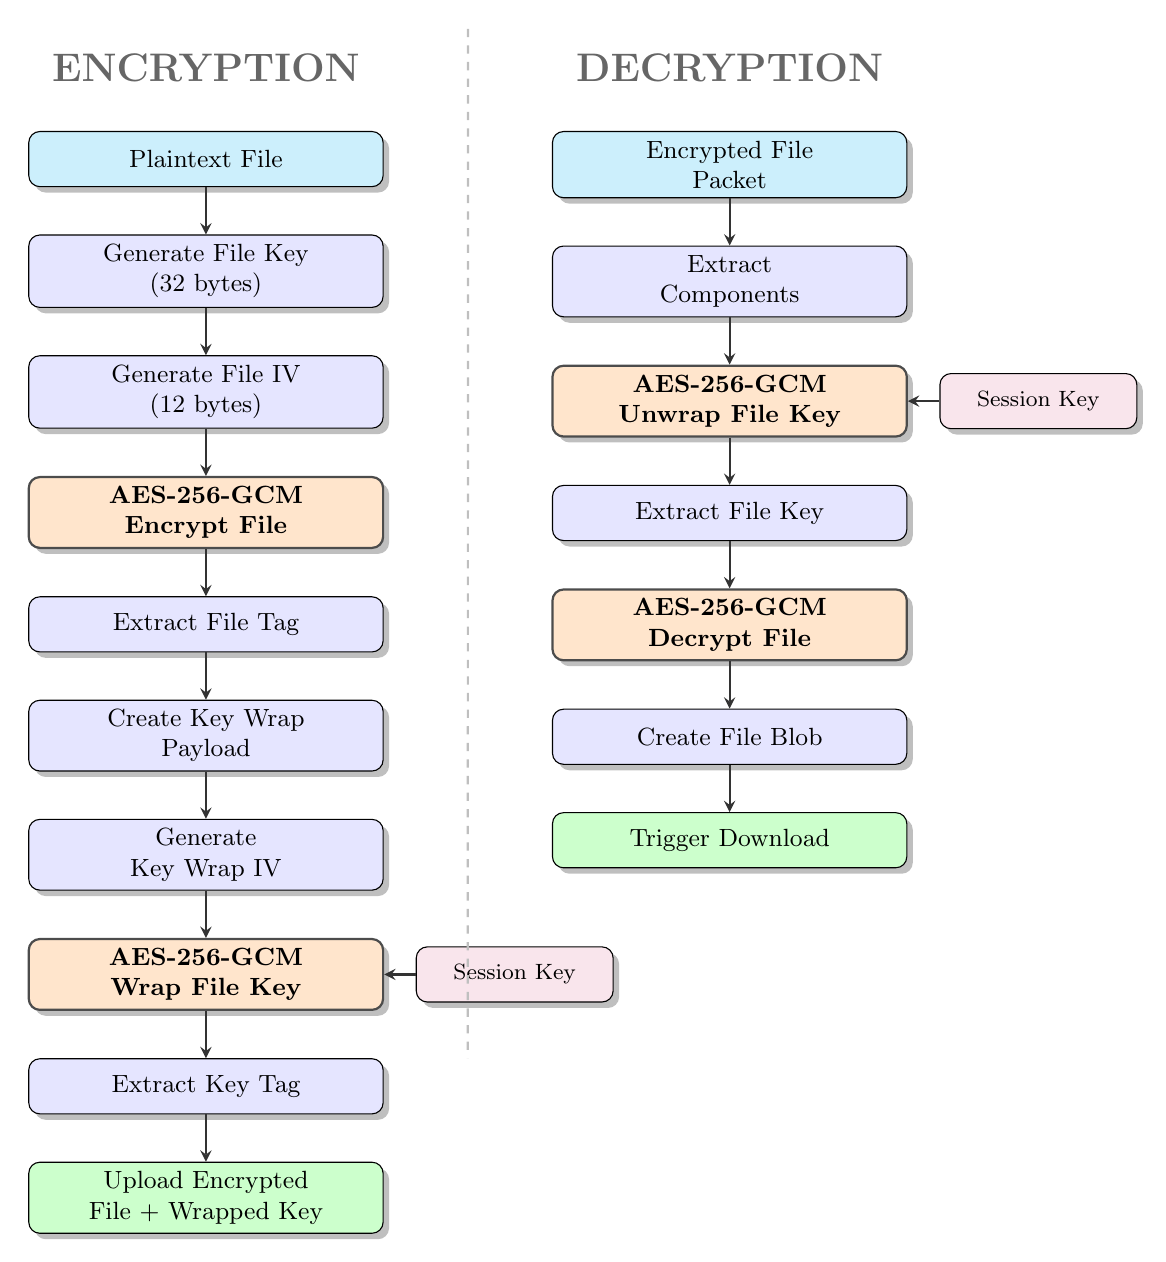
\begin{tikzpicture}[
    node distance=0.6cm and 1cm,
    process/.style={rectangle, draw, minimum width=4.5cm, minimum height=0.7cm, align=center, fill=blue!10, rounded corners, drop shadow, font=\small},
    input/.style={rectangle, draw, minimum width=4.5cm, minimum height=0.7cm, align=center, fill=cyan!20, rounded corners, drop shadow, font=\small},
    output/.style={rectangle, draw, minimum width=4.5cm, minimum height=0.7cm, align=center, fill=green!20, rounded corners, drop shadow, font=\small},
    crypto/.style={rectangle, draw=black!70, thick, minimum width=4.5cm, minimum height=0.8cm, align=center, fill=orange!20, rounded corners, drop shadow, font=\small\bfseries},
    arrow/.style={->, >=stealth, thick, color=black!80},
    section_label/.style={font=\Large\bfseries, align=center, text=gray!80!black}
]

    % ============================================================
    % LEFT COLUMN: ENCRYPTION
    % ============================================================
    \node[section_label] (enc-label) {ENCRYPTION};
    
    \node[input, below=0.5cm of enc-label] (file) {Plaintext File};
    \node[process, below=of file] (genfilekey) {Generate File Key\\(32 bytes)};
    \node[process, below=of genfilekey] (genfileiv) {Generate File IV\\(12 bytes)};
    \node[crypto, below=of genfileiv] (encfile) {AES-256-GCM\\Encrypt File};
    \node[process, below=of encfile] (extract1) {Extract File Tag};
    \node[process, below=of extract1] (genkeywrap) {Create Key Wrap\\Payload};
    \node[process, below=of genkeywrap] (genkeyiv) {Generate\\Key Wrap IV};
    \node[crypto, below=of genkeyiv] (enckey) {AES-256-GCM\\Wrap File Key};
    \node[process, below=of enckey] (extract2) {Extract Key Tag};
    \node[output, below=of extract2] (uploadfile) {Upload Encrypted\\File + Wrapped Key};

    % Connections Left
    \draw[arrow] (file) -- (genfilekey);
    \draw[arrow] (genfilekey) -- (genfileiv);
    \draw[arrow] (genfileiv) -- (encfile);
    \draw[arrow] (encfile) -- (extract1);
    \draw[arrow] (extract1) -- (genkeywrap);
    \draw[arrow] (genkeywrap) -- (genkeyiv);
    \draw[arrow] (genkeyiv) -- (enckey);
    \draw[arrow] (enckey) -- (extract2);
    \draw[arrow] (extract2) -- (uploadfile);

    % Session Key Input (Left Side)
    \node[input, right=0.4cm of enckey, fill=purple!10, font=\footnotesize, minimum width=2.5cm] (sesskey1) {Session Key};
    \draw[arrow] (sesskey1) -- (enckey);

    % ============================================================
    % RIGHT COLUMN: DECRYPTION
    % ============================================================
    % Reduced spacing from 7cm to 1.5cm to fit on page
    \node[section_label, right=2.5cm of enc-label] (dec-label) {DECRYPTION};

    \node[input, below=0.5cm of dec-label] (recfile) {Encrypted File\\Packet};
    \node[process, below=of recfile] (extract3) {Extract\\Components};
    
    % Aligning logically with the wrap steps
    \node[crypto, below=of extract3] (deckey) {AES-256-GCM\\Unwrap File Key};
    \node[process, below=of deckey] (extract4) {Extract File Key};
    \node[crypto, below=of extract4] (decfile) {AES-256-GCM\\Decrypt File};
    \node[process, below=of decfile] (createblob) {Create File Blob};
    \node[output, below=of createblob] (download) {Trigger Download};

    % Connections Right
    \draw[arrow] (recfile) -- (extract3);
    \draw[arrow] (extract3) -- (deckey);
    \draw[arrow] (deckey) -- (extract4);
    \draw[arrow] (extract4) -- (decfile);
    \draw[arrow] (decfile) -- (createblob);
    \draw[arrow] (createblob) -- (download);

    % Session Key Input (Right Side)
    \node[input, right=0.4cm of deckey, fill=purple!10, font=\footnotesize, minimum width=2.5cm] (sesskey2) {Session Key};
    \draw[arrow] (sesskey2) -- (deckey);

    % ============================================================
    % BACKGROUNDS & LABELS
    % ============================================================
    
    % Draw a separator line centered between columns
    \coordinate (top-mid) at ($(enc-label.east)!0.5!(dec-label.west)$);
    \coordinate (bot-mid) at ($(uploadfile.east)!0.5!(download.west)$);
    
    \draw[dashed, thick, gray!50] ($(top-mid) + (0, 0.5)$) -- ($(bot-mid) + (0, -0.5)$);

    

\end{tikzpicture}
\caption{File Encryption and Decryption Workflow}
\label{fig:file-encrypt-decrypt}
\end{figure}


\newpage
%==============================================================================
% SECTION 6: ATTACK DEMONSTRATIONS
%==============================================================================
\section{Attack Demonstrations}
\label{sec:attacks}

\threatbox{Attack Demonstrations Overview}{
This section demonstrates two critical attack vectors and how the protocol defends against them:\\[4pt]
\textbf{1. Man-in-the-Middle (MITM):} Attacker intercepts and replaces ephemeral keys to position themselves between communicating parties. Defense: Digital signature authentication of ephemeral ECDH keys.\\[4pt]
\textbf{2. Replay Attack:} Attacker captures encrypted messages and resubmits them later. Defense: Three-layer protection combining timestamp validation, nonce deduplication, and sequence counters.
}

\subsection{Man-in-the-Middle (MITM) Attack Demonstration}
\label{sec:mitm-demo}

\subsubsection{Overview}

The application includes an interactive demonstration of how man-in-the-middle attacks work and how digital signatures prevent them. This section explains two scenarios: one where the attack succeeds (unsigned key exchange) and one where it fails (signed key exchange).

\subsubsection{Vulnerable Scenario: Unsigned ECDH Key Exchange}

\threatbox{Attack Success Condition}{
Without signature verification, an attacker (Mallory) can intercept and replace cryptographic keys by substituting her own keys while claiming to be the sender. This allows her to establish separate shared secrets with each party and intercept/modify all communications.
}

\begin{enumerate}
    \item \textbf{Key Generation Phase}: Alice and Bob each generate ephemeral ECDH P-256 key pairs. These keys are sent to each other but are not digitally signed.
    
    \item \textbf{Attacker Intercepts Alice's Key}: Mallory intercepts Alice's ECDH public key while it is being transmitted to Bob. Instead of forwarding Alice's authentic key to Bob, Mallory generates her own ECDH key pair and sends it to Bob while claiming to be Alice.
    
    \item \textbf{Attacker Intercepts Bob's Key}: When Bob sends his ECDH public key back, Mallory intercepts it and sends her own ECDH public key to Alice, claiming to be Bob.
    
    \item \textbf{Two Independent Shared Secrets}: Mallory now possesses two separate shared secrets:
    \begin{itemize}
        \item Shared secret 1: Derived from Alice's private ECDH key and Mallory's public ECDH key
        \item Shared secret 2: Derived from Bob's private ECDH key and Mallory's public ECDH key
    \end{itemize}
    
    \item \textbf{Message Interception and Relay}: When Alice sends an encrypted message, she encrypts it with Shared Secret 1 (which Mallory also possesses). Mallory decrypts the message, reads its contents, re-encrypts it with Shared Secret 2, and forwards it to Bob. The reverse happens for messages from Bob to Alice.
    
    \item \textbf{Transparency to Victims}: Neither Alice nor Bob realizes that a third party is reading their messages. The communication appears normal to both parties, but Mallory can read and potentially modify all communications.
    
    \item \textbf{Attack Outcome}: Mallory achieves complete compromise of message confidentiality and integrity without being detected.
\end{enumerate}

\subsubsection{Protected Scenario: Signed ECDH Key Exchange}

\securitybox{Attack Prevention Mechanism}{
With digital signatures authenticating ephemeral ECDH public keys, the attacker faces an impossible cryptographic dilemma: either forward the authentic key (losing ability to intercept) or forge a signature (which fails verification and exposes the attack). No third option exists.
}

\begin{enumerate}
    \item \textbf{Signature Requirement}: In the secure protocol (Phase 2 of the key exchange), each party cryptographically signs their ephemeral ECDH public key using their long-term identity private key (RSA-PSS or ECDSA P-256).
    
    \item \textbf{Mallory's Dilemma}: When Mallory attempts the attack, she faces an impossible choice:
    \begin{itemize}
        \item \textbf{Option A - Forward Authentic Key and Signature}: If Mallory forwards Alice's authentic ECDH public key and signature to Bob without modification, Bob verifies the signature using Alice's published identity public key. Verification succeeds because Alice signed the key correctly. Bob accepts it and the key exchange proceeds with the real Alice. However, Mallory is left unable to decrypt because she doesn't possess Alice's ECDH private key. The attack fails because Mallory cannot read the messages.
        
        \item \textbf{Option B - Substitute Key with Forged Signature}: If Mallory generates her own ECDH key and tries to send it to Bob with a forged signature, Bob verifies the signature using Alice's published identity public key. Since Alice never signed Mallory's ECDH key, the signature verification fails. Bob detects the forged signature and immediately aborts the key exchange. The attack is detected and prevented before any session key is established.
    \end{itemize}
    
    \item \textbf{Fundamental Limitation}: Mallory cannot create a valid signature of her own ECDH key using Alice's private key (because she doesn't possess it), and she cannot forge Alice's signature on her key. This cryptographic impossibility defeats the attack.
    
    \item \textbf{Attack Detection}: When signature verification fails, the system logs a security event (\texttt{MITM\_ATTACK\_DETECTED}) and terminates the key exchange. The user is informed that the session establishment has failed and can retry.
    
    \item \textbf{Attack Outcome}: Mallory cannot establish herself between Alice and Bob without being detected. The attack fails completely.
\end{enumerate}

\subsubsection{Key Insight: Authentication of Ephemeral Keys}

The critical difference between the vulnerable and secure scenarios is \textbf{who authenticates the ephemeral ECDH public key}. 

In the vulnerable scenario, Alice and Bob have no way to verify that the ECDH public key they received was actually generated by their peer. Mallory exploits this by substituting her own key.

In the secure scenario, each ECDH public key is digitally signed by the sender's long-term identity key. The receiver verifies this signature using the sender's published identity public key. This signature creates an unforgeable binding between the ephemeral key and the sender's identity. An attacker cannot forge this signature without possessing the sender's private key, making the substitution attack impossible.

\subsubsection{Demonstration Implementation}

The application provides an interactive MITM demo page with the following features:

\begin{itemize}
    \item \textbf{Unsigned Demo Mode}: Users can generate ECDH keys without signatures and simulate Mallory's key substitution. The demo shows how the attack succeeds transparently, with Mallory able to view messages exchanged between Alice and Bob.
    
    \item \textbf{Signed Demo Mode}: Users can generate ECDH keys with signatures. The demo shows that when Mallory attempts key substitution, signature verification fails and the key exchange is aborted.
    
    \item \textbf{Visual Flow}: Sequence diagrams illustrate the key exchange flow in both scenarios, clearly showing where signature verification occurs and why it prevents the attack.
    
    \item \textbf{Audit Log Evidence}: Both scenarios generate audit log entries showing the difference between successful key exchange (with valid signatures) and failed key exchange (with invalid signatures).
\end{itemize}

---

\subsection{Replay Attack Demonstration}
\label{sec:replay-demo}

\subsubsection{Overview}

The application implements three independent replay protection mechanisms that work together to prevent attackers from resubmitting captured messages. This section explains how each mechanism works and why all three are necessary.

\subsubsection{Replay Attack Concept}

\threatbox{Attack Description}{
An attacker captures a valid encrypted message and resubmits it later, attempting to force the receiver to process the identical message twice. This can cause duplicate message delivery, repeated transactions, bandwidth waste, and message ordering violations.
}

\begin{itemize}
    \item Duplicate message delivery (disrupting conversation flow)
    \item Repeated file transfers (wasting bandwidth)
    \item Repeated transactions (in a payment system, double-charging)
    \item Loss of message ordering guarantees
\end{itemize}

\subsubsection{Layer 1: Timestamp-Based Replay Protection}

\textbf{Mechanism}:
Each message includes a server-generated timestamp indicating when it was created. The server validates that incoming message timestamps fall within a 30-second window (±30 seconds from current server time).

\textbf{Protection Window}:
\begin{itemize}
    \item Messages with timestamps more than 30 seconds in the past are rejected as stale
    \item Messages with timestamps more than 30 seconds in the future are rejected as invalid (clock skew tolerance)
    \item Only messages within the current 30-second window are accepted
\end{itemize}

\textbf{Justification for 30-Second Window}:
\begin{itemize}
    \item \textbf{Network Latency}: Most network messages complete within 1-5 seconds, leaving 25+ seconds for clock skew tolerance
    \item \textbf{Clock Skew}: Operating system clocks can drift, and users might not synchronize with NTP. 30 seconds accommodates typical clock drift
    \item \textbf{Attack Window}: Limits the time window during which a captured message can be replayed
\end{itemize}

\textbf{Limitation}:
Timestamp protection alone is vulnerable to attacks within the 30-second window. An attacker who captures a message at T=1000 can replay it at any time up to T=1030, still passing timestamp validation.

\subsubsection{Layer 2: Nonce-Based Replay Protection}

\textbf{Mechanism}:
Each message includes a unique 128-bit random nonce (number used once). The server maintains a list of recently seen nonces per conversation. If a nonce is received twice, the message is rejected.

\textbf{Nonce Management}:
\begin{itemize}
    \item When a message arrives, the server checks if its nonce is in the \texttt{recentNonces} list
    \item If the nonce is found (duplicate), the message is rejected as a replay
    \item If the nonce is new, it is added to the \texttt{recentNonces} list
    \item Old nonces (older than 30 seconds) are automatically cleaned up to prevent unbounded memory growth
\end{itemize}

\textbf{Security of Nonces}:
With 128-bit random nonces, there are $2^{128}$ possible values. The probability of accidental collision is negligible. For an attacker to bypass nonce protection, they must capture and replay within the 30-second window before the nonce is cleaned up.

\textbf{Limitation}:
Nonce protection alone requires server-side state management. If the server crashes or restarts and loses the \texttt{recentNonces} list, previously seen nonces may be accepted again. Additionally, nonces must be cleaned up before being reused, which requires careful implementation.

\subsubsection{Layer 3: Sequence Number-Based Replay Protection}

\textbf{Mechanism}:
Each message from a sender includes a sequence number (monotonically increasing counter). The server tracks the last sequence number received from each sender. If a message's sequence number does not exceed the last recorded sequence, the message is rejected.

\textbf{Sequence Validation Logic}:
\begin{itemize}
    \item Alice sends message M1 with sequence=1. Server stores: \texttt{lastSequenceFromAlice = 1}
    \item Alice sends message M2 with sequence=2. Server stores: \texttt{lastSequenceFromAlice = 2}
    \item Attacker replays M1 with sequence=1. Server checks: 1 > 2? No. Message rejected
    \item Attacker replays M2 with sequence=2. Server checks: 2 > 2? No. Message rejected
\end{itemize}

\textbf{Ordering Guarantee}:
Sequence numbers enforce strict ordering. Out-of-order messages (where sequence < lastSequence) are automatically rejected, preventing attackers from reordering or duplicating messages.

\textbf{Limitation}:
Sequence protection alone doesn't prevent immediate replays. If Alice sends M1 with sequence=1 at T=1000, and Mallory captures and immediately replays M1 with sequence=1 at T=1005, the sequence number is identical. The attacker must wait for the next message to increment the sequence, at which point earlier sequences can no longer be accepted.

\subsubsection{Why All Three Layers Are Necessary}

\securitybox{Defense-in-Depth Strategy}{
\textbf{Layer 1 (Timestamp):} Rejects messages older than 30 seconds, limiting attack window for stale captures\\[3pt]
\textbf{Layer 2 (Nonce):} Prevents duplicate message within the 30-second window, catches immediate replays\\[3pt]
\textbf{Layer 3 (Sequence):} Enforces ordering and prevents out-of-order replays, provides long-term protection\\[3pt]
\textbf{Combined Effect:} An attacker must defeat all three mechanisms simultaneously to succeed, which is cryptographically infeasible.
}
\newpage
\section{Audit Logs and Evidence}
\label{sec:logs}

\subsection{Audit Logging System}

The application implements comprehensive security event logging to track all security-relevant operations.

\subsubsection{Logged Event Types}

\begin{table}[H]
\centering
\begin{tabular}{@{}llp{5cm}@{}}
\toprule
\textbf{Category} & \textbf{Event Type} & \textbf{Description} \\ \midrule
Authentication & LOGIN\_SUCCESS & User successfully authenticated \\
 & LOGOUT & User logged out \\
 & IDENTITY\_KEY\_GENERATED & New identity key pair created \\
 & IDENTITY\_KEY\_LOADED & Private key decrypted from storage \\
\midrule
Key Exchange & KEY\_EXCHANGE\_REQUEST\_SENT & Initiator sent ECDH request \\
 & KEY\_EXCHANGE\_REQUEST\_RECEIVED & Responder received request \\
 & KEY\_EXCHANGE\_RESPONSE\_SENT & Responder sent signed response \\
 & KEY\_EXCHANGE\_RESPONSE\_RECEIVED & Initiator received response \\
 & KEY\_CONFIRM\_A\_SENT & First confirmation sent \\
 & KEY\_CONFIRM\_A\_RECEIVED & First confirmation received \\
 & KEY\_CONFIRM\_B\_SENT & Second confirmation sent \\
 & KEY\_CONFIRM\_B\_RECEIVED & Second confirmation received \\
 & SESSION\_ESTABLISHED & Session key successfully derived \\
\midrule
Security & REPLAY\_ATTACK\_BLOCKED & Replay attempt detected \\
 & MITM\_ATTACK\_DETECTED & Signature verification failed \\
 & SIGNATURE\_VERIFICATION\_FAILED & Invalid signature detected \\
\midrule
File Operations & ENCRYPTED\_FILE\_UPLOAD & File encrypted and uploaded \\
 & FILE\_DECRYPTED & File successfully decrypted \\
\bottomrule
\end{tabular}
\caption{Security Event Types}
\label{tab:event-types}
\end{table}

\subsubsection{Sample Audit Log Entries}

\begin{lstlisting}[caption=Example Audit Log - Successful Key Exchange]
[
  {
    "username": "shoukat_",
    "eventType": "KEY_EXCHANGE_REQUEST_SENT",
    "timestamp": "2025-11-30T10:15:23.456Z",
    "details": {
      "peer": "hashim_",
      "description": "Initiated key exchange with hashim_"
    }
  },
  {
    "username": "hashim_",
    "eventType": "KEY_EXCHANGE_REQUEST_RECEIVED",
    "timestamp": "2025-11-30T10:15:24.123Z",
    "details": {
      "initiator": "shoukat_",
      "signatureVerified": true
    }
  },
  {
    "username": "hashim_",
    "eventType": "KEY_EXCHANGE_RESPONSE_SENT",
    "timestamp": "2025-11-30T10:15:25.789Z",
    "details": {
      "peer": "shoukat_",
      "description": "Sent signed ECDH response"
    }
  },
  {
    "username": "shoukat_",
    "eventType": "KEY_EXCHANGE_RESPONSE_RECEIVED",
    "timestamp": "2025-11-30T10:15:26.234Z",
    "details": {
      "peer": "hashim_",
      "signatureVerified": true
    }
  },
  {
    "username": "shoukat_",
    "eventType": "SESSION_ESTABLISHED",
    "timestamp": "2025-11-30T10:15:28.567Z",
    "details": {
      "peer": "hashim_",
      "confirmationsExchanged": true
    }
  },
  {
    "username": "hashim_",
    "eventType": "SESSION_ESTABLISHED",
    "timestamp": "2025-11-30T10:15:28.890Z",
    "details": {
      "peer": "shoukat_",
      "confirmationsExchanged": true
    }
  }
]
\end{lstlisting}

\begin{lstlisting}[caption=Example Audit Log - MITM Attack Detection]
[
  {
    "username": "shoukat_",
    "eventType": "MITM_ATTACK_DETECTED",
    "timestamp": "2025-11-30T10:20:15.123Z",
    "details": {
      "description": "Signature verification failed in secure demo",
      "peer": "hashim_",
      "action": "Key exchange aborted"
    }
  }
]
\end{lstlisting}

\begin{lstlisting}[caption=Example Audit Log - Replay Attack Blocked]
[
  {
    "username": "hashim_",
    "eventType": "REPLAY_ATTACK_BLOCKED",
    "timestamp": "2025-11-30T10:25:30.456Z",
    "details": {
      "reason": "Duplicate nonce detected",
      "sender": "shoukat_",
      "nonce": "a1b2c3d4e5f6...",
      "action": "Message rejected"
    }
  }
]
\end{lstlisting}

%==============================================================================
% SECTION 8: SYSTEM ARCHITECTURE
%==============================================================================
\section{System Architecture}
\label{sec:architecture}

\subsection{High-Level Architecture}

\begin{figure}[H]
\centering
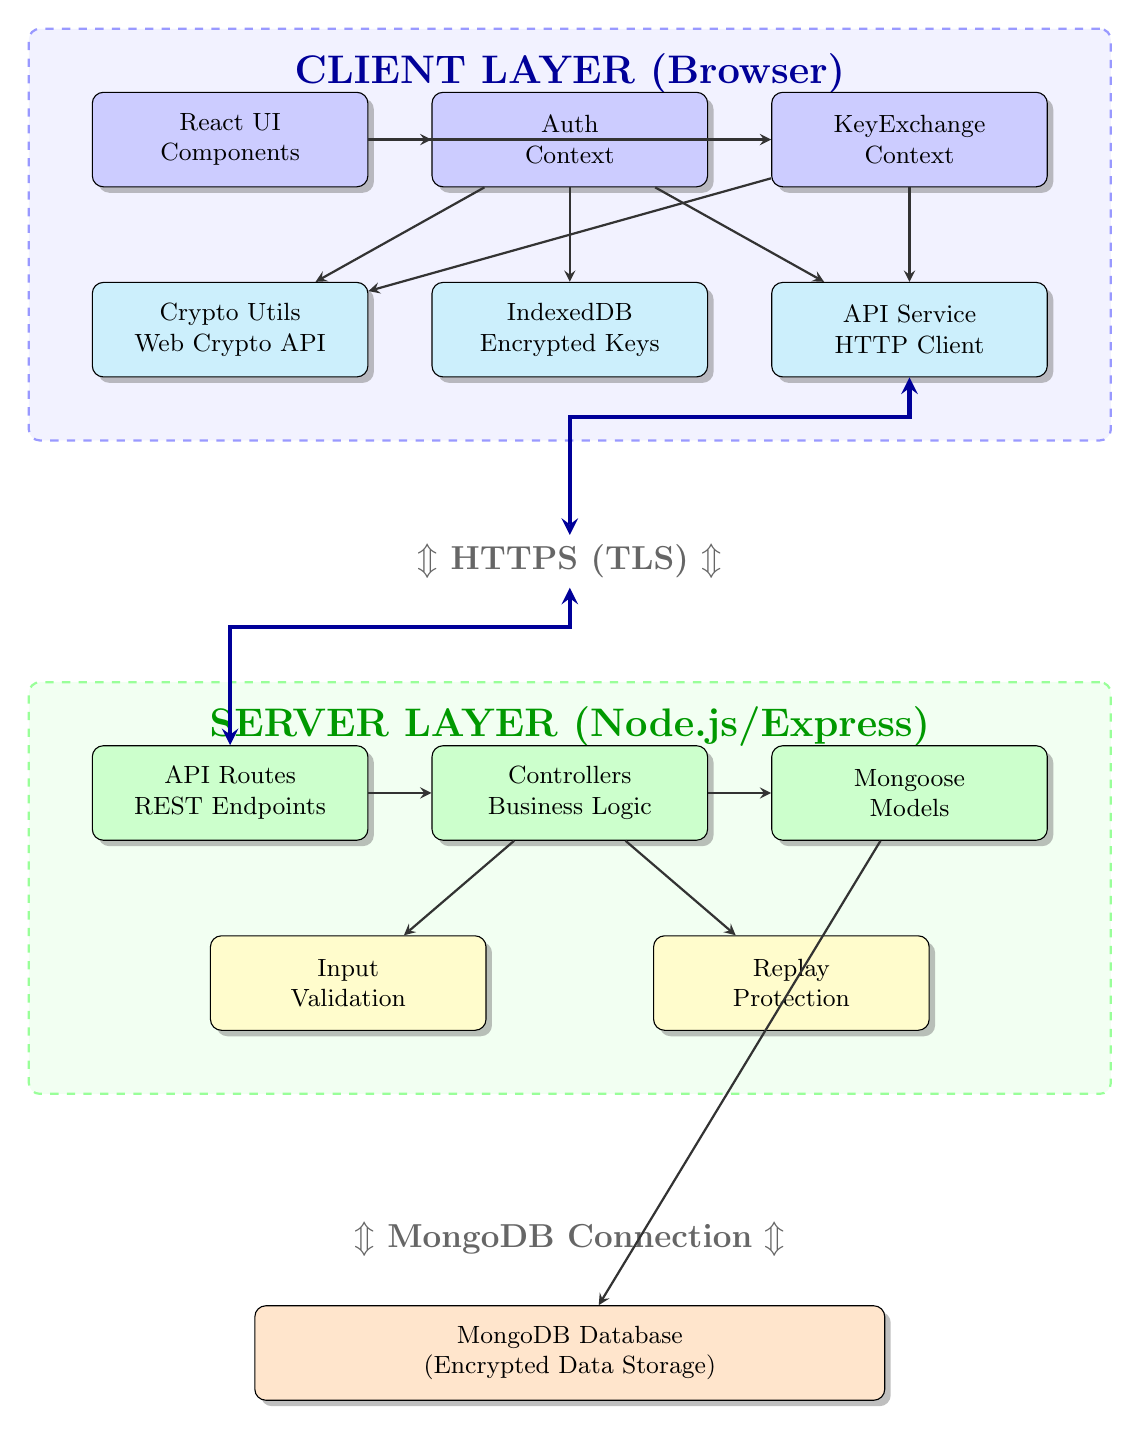
\begin{tikzpicture}[
    node distance=1.2cm and 0.8cm, % Increased global spacing
    component/.style={rectangle, draw, minimum width=3.5cm, minimum height=1.2cm, align=center, rounded corners, drop shadow, fill=white, font=\small},
    layerlabel/.style={font=\Large\bfseries, anchor=north, yshift=-0.2cm},
    arrow/.style={->, >=stealth, thick, color=black!80},
    dblarrow/.style={<->, >=stealth, ultra thick, color=blue!60!black}
]

    % --- Client Components ---
    % Top Row
    \node[component, fill=blue!20] (auth-ctx) {Auth\\Context};
    \node[component, fill=blue!20, left=of auth-ctx] (ui) {React UI\\Components};
    \node[component, fill=blue!20, right=of auth-ctx] (kex-ctx) {KeyExchange\\Context};

    % Bottom Row (Client)
    \node[component, fill=cyan!20, below=of auth-ctx] (indexdb) {IndexedDB\\Encrypted Keys};
    \node[component, fill=cyan!20, left=of indexdb] (crypto) {Crypto Utils\\Web Crypto API};
    \node[component, fill=cyan!20, right=of indexdb] (api-svc) {API Service\\HTTP Client};

    % Client Layer Box
    \begin{scope}[on background layer]
        \node[draw=blue!40, fill=blue!5, dashed, thick, rounded corners, fit=(ui) (kex-ctx) (crypto) (api-svc) (indexdb) (auth-ctx), inner sep=0.8cm] (client-layer) {};
        \node[layerlabel, text=blue!60!black] at (client-layer.north) {CLIENT LAYER (Browser)};
    \end{scope}

    % --- Network Gap ---
    % Increased spacing here
    \node[below=2.0cm of indexdb, font=\large\bfseries, text=gray!80!black] (network) {$\Updownarrow$ HTTPS (TLS) $\Updownarrow$};

    % --- Server Components ---
    % Top Row (Server) - Aligned relative to network/client
    % Increased spacing here as well
    \node[component, fill=green!20, below=2.0cm of network] (controllers) {Controllers\\Business Logic};
    \node[component, fill=green!20, left=of controllers] (routes) {API Routes\\REST Endpoints};
    \node[component, fill=green!20, right=of controllers] (models) {Mongoose\\Models};

    % Bottom Row (Server)
    % Positioning these centered under the top row
    \node[component, fill=yellow!20, below=of routes, xshift=1.5cm] (validation) {Input\\Validation};
    \node[component, fill=yellow!20, below=of models, xshift=-1.5cm] (replay-check) {Replay\\Protection};

    % Server Layer Box
    \begin{scope}[on background layer]
        \node[draw=green!40, fill=green!5, dashed, thick, rounded corners, fit=(routes) (models) (validation) (replay-check) (controllers), inner sep=0.8cm] (server-layer) {};
        \node[layerlabel, text=green!60!black] at (server-layer.north) {SERVER LAYER (Node.js/Express)};
    \end{scope}

    % --- Database ---
    % Increased spacing here
    \node[below=1.5cm of server-layer, font=\large\bfseries, text=gray!80!black] (db-label) {$\Updownarrow$ MongoDB Connection $\Updownarrow$};
    \node[component, below=0.5cm of db-label, fill=orange!20, minimum width=8cm] (mongodb) {MongoDB Database\\(Encrypted Data Storage)};

    % --- Connections ---
    % Client Internal
    \draw[arrow] (ui) -- (auth-ctx);
    \draw[arrow] (ui) -- (kex-ctx);
    
    \draw[arrow] (auth-ctx) -- (crypto);
    \draw[arrow] (kex-ctx) -- (crypto);
    
    \draw[arrow] (auth-ctx) -- (indexdb);
    
    \draw[arrow] (auth-ctx) -- (api-svc);
    \draw[arrow] (kex-ctx) -- (api-svc);

    % Network
    \draw[dblarrow] (api-svc.south) -- ++(0,-0.5) -| (network.north);
    \draw[dblarrow] (network.south) |- ++(0,-0.5) -| (routes.north);

    % Server Internal
    \draw[arrow] (routes) -- (controllers);
    \draw[arrow] (controllers) -- (models);
    \draw[arrow] (controllers) -- (validation);
    \draw[arrow] (controllers) -- (replay-check);

    % Database
    \draw[arrow] (models) -- (mongodb);

\end{tikzpicture}
\caption{High-Level System Architecture}
\label{fig:architecture}
\end{figure}

\subsection{Component Responsibilities}

\subsubsection{Client-Side Components}

\begin{table}[H]
\centering
\small
\begin{tabular}{@{}lp{8cm}@{}}
\toprule
\textbf{Component} & \textbf{Responsibilities} \\ \midrule
\texttt{AuthContext} & User authentication, identity key generation/loading, private key encryption/decryption, session management \\
\texttt{KeyExchangeContext} & ECDH key generation, key exchange protocol, session key derivation, message encryption/decryption, file operations \\
\texttt{cryptoUtils.js} & Web Crypto API wrappers, all cryptographic operations (signing, verification, encryption, key derivation) \\
\texttt{indexedDBUtils.js} & Persistent storage of encrypted private keys \\
\texttt{apiService.js} & HTTP communication with backend, axios instance configuration \\
\bottomrule
\end{tabular}
\caption{Client Component Responsibilities}
\label{tab:client-components}
\end{table}

\subsubsection{Server-Side Components}

\begin{table}[H]
\centering
\small
\begin{tabular}{@{}lp{8cm}@{}}
\toprule
\textbf{Component} & \textbf{Responsibilities} \\ \midrule
\texttt{authController} & User registration, login, password hashing, public key storage \\
\texttt{keyExchangeController} & Key exchange request/response/confirm handling, state management \\
\texttt{messageController} & Encrypted message storage/retrieval, replay protection validation \\
\texttt{fileController} & Encrypted file upload/download, metadata management \\
\texttt{auditController} & Security event logging, audit log retrieval \\
\texttt{Conversation} & Replay protection state (nonces, sequences, timestamps) \\
\bottomrule
\end{tabular}
\caption{Server Component Responsibilities}
\label{tab:server-components}
\end{table}

\subsection{Data Flow Diagrams}

\subsubsection{Registration Data Flow}

\begin{figure}[H]
\centering
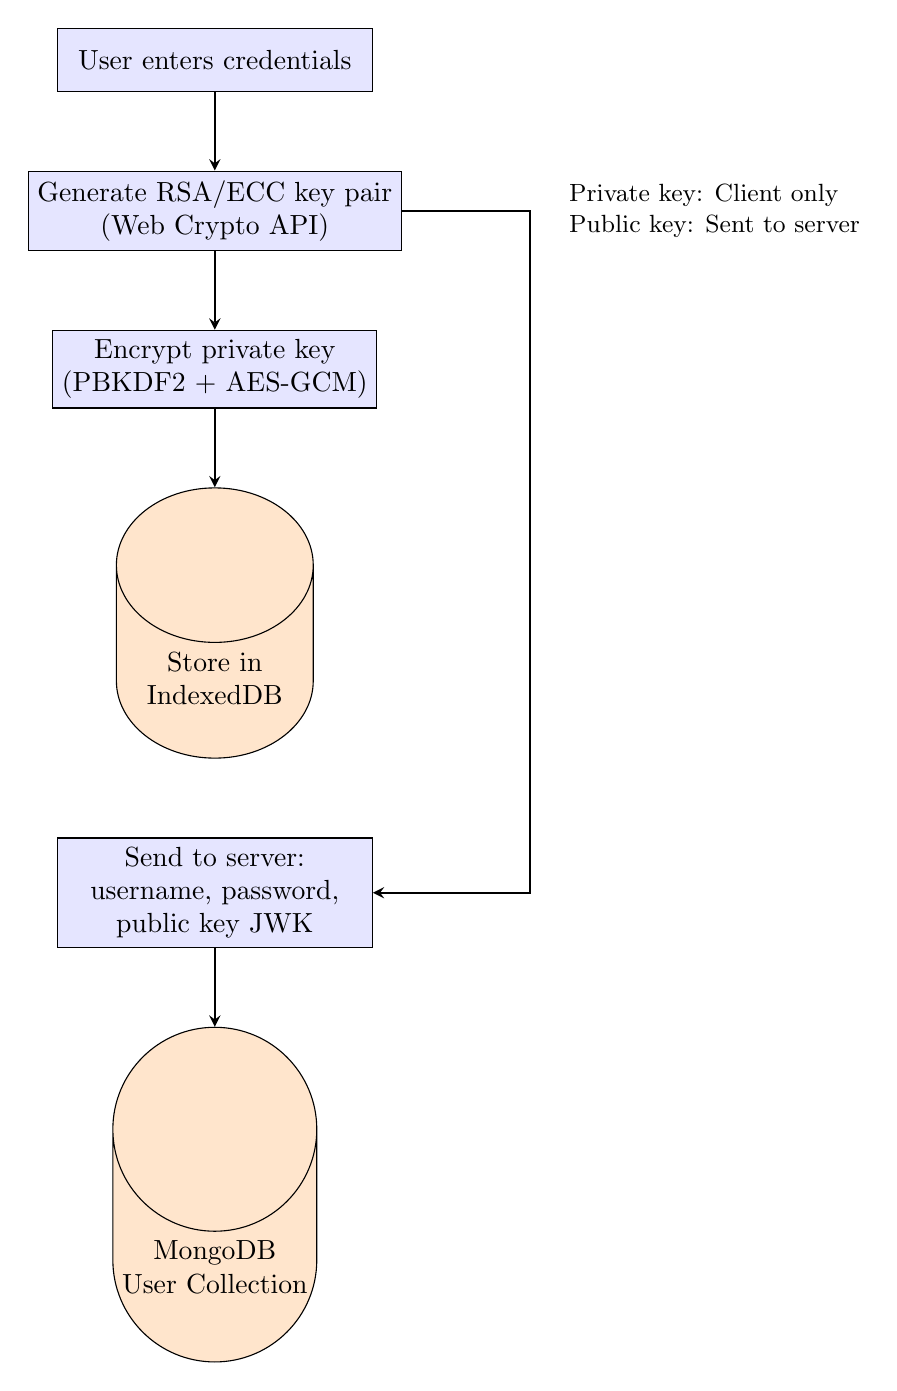
\begin{tikzpicture}[
    node distance=1cm,
    process/.style={rectangle, draw, minimum width=4cm, minimum height=0.8cm, align=center, fill=blue!10},
    storage/.style={cylinder, draw, shape border rotate=90, minimum width=2.5cm, minimum height=1cm, align=center, fill=orange!20},
    arrow/.style={->, >=stealth, thick}
]

\node[process] (input) {User enters credentials};
\node[process, below=of input] (gen-keys) {Generate RSA/ECC key pair\\(Web Crypto API)};
\node[process, below=of gen-keys] (encrypt) {Encrypt private key\\(PBKDF2 + AES-GCM)};
\node[storage, below=of encrypt] (indexdb) {Store in\\IndexedDB};
\node[process, below=of indexdb] (send) {Send to server:\\username, password,\\public key JWK};
\node[storage, below=of send] (mongo) {MongoDB\\User Collection};

\draw[arrow] (input) -- (gen-keys);
\draw[arrow] (gen-keys) -- (encrypt);
\draw[arrow] (encrypt) -- (indexdb);
\draw[arrow] (gen-keys) -- ++(4,0) |- (send);
\draw[arrow] (send) -- (mongo);

\node[right=2cm of gen-keys, align=left, font=\small] (note1) {
    Private key: Client only\\
    Public key: Sent to server
};

\end{tikzpicture}
\caption{Registration Data Flow}
\label{fig:registration-flow}
\end{figure}

\subsubsection{Secure Communication Data Flow}

\begin{figure}[H]
\centering
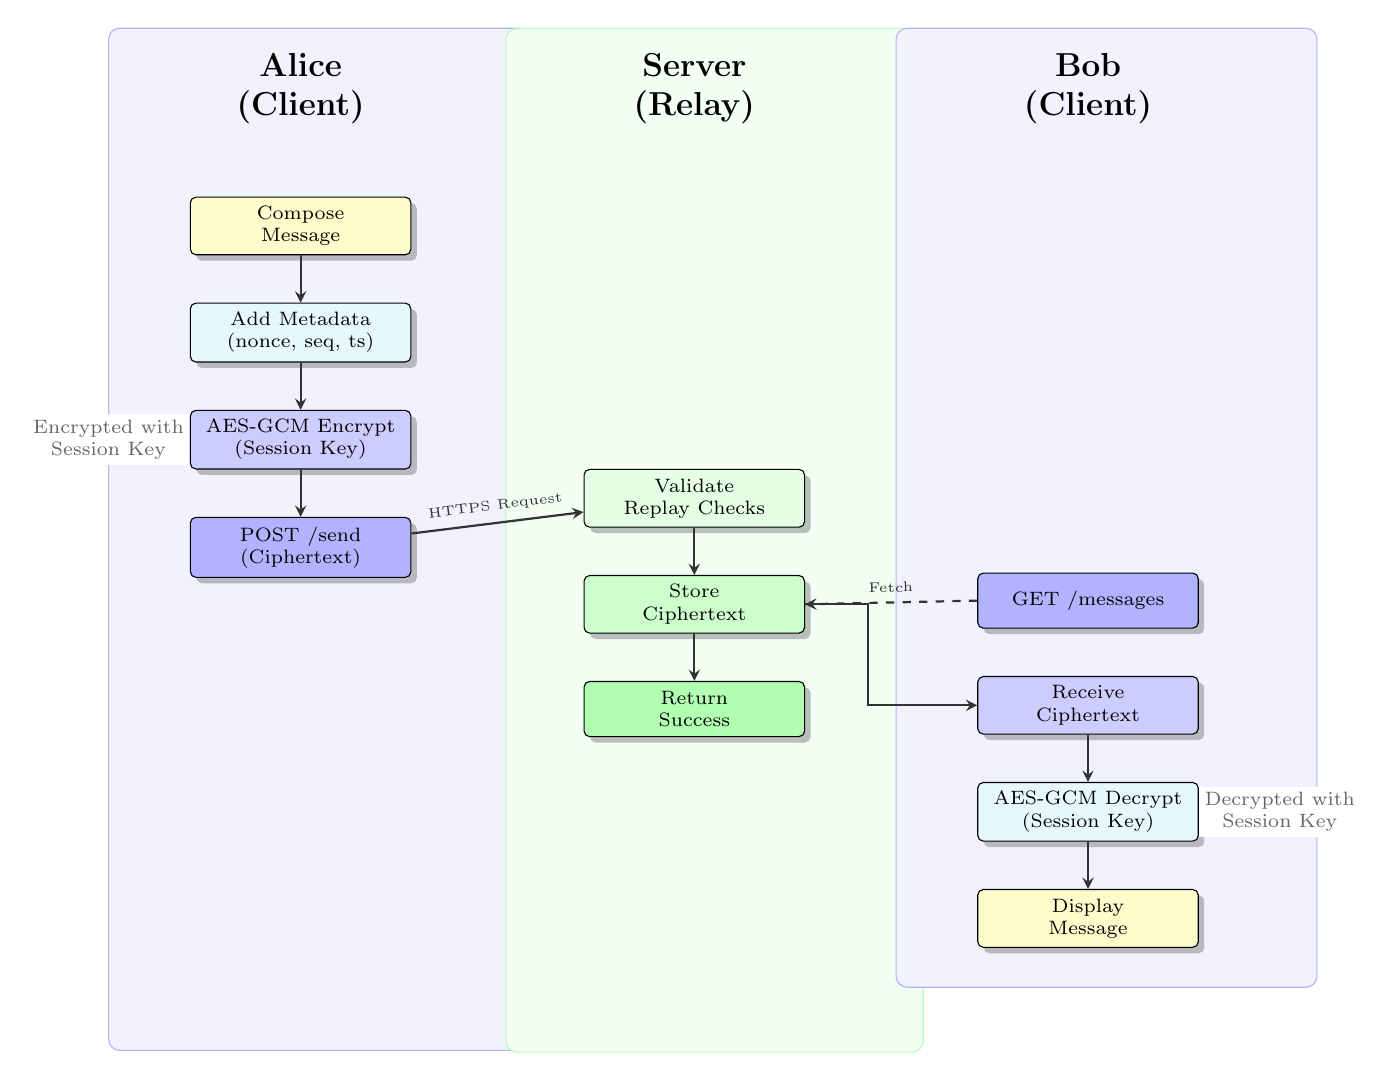
\begin{tikzpicture}[
    node distance=0.6cm,
    colheader/.style={font=\bfseries\large, align=center},
    msgstep/.style={rectangle, draw, minimum width=2.8cm, minimum height=0.7cm, align=center, font=\scriptsize, drop shadow, fill=white, rounded corners=2pt},
    arrow/.style={->, >=stealth, thick, color=black!80},
    note/.style={font=\scriptsize, color=gray!80!black, align=center, fill=white, inner sep=2pt}
]

    % --- Actor Columns ---
    % Alice
    \node[colheader] (h_alice) at (0,0) {Alice\\(Client)};
    
    % Server
    \node[colheader] (h_server) at (5,0) {Server\\(Relay)};
    
    % Bob
    \node[colheader] (h_bob) at (10,0) {Bob\\(Client)};

    % --- Alice's Steps ---
    \node[msgstep, fill=yellow!20, below=0.8cm of h_alice] (a1) {Compose\\Message};
    \node[msgstep, fill=cyan!10, below=of a1] (a2) {Add Metadata\\(nonce, seq, ts)};
    \node[msgstep, fill=blue!20, below=of a2] (a3) {AES-GCM Encrypt\\(Session Key)};
    \node[msgstep, fill=blue!30, below=of a3] (a4) {POST /send\\(Ciphertext)};

    % --- Server's Steps ---
    % Align s1 roughly with a4's output
    \node[msgstep, fill=green!10] (s1) at (5, -5.2) {Validate\\Replay Checks};
    \node[msgstep, fill=green!20, below=of s1] (s2) {Store\\Ciphertext};
    \node[msgstep, fill=green!30, below=of s2] (s3) {Return\\Success};

    % --- Bob's Steps ---
    % Bob polls/receives later
    \node[msgstep, fill=blue!30] (b1) at (10, -6.5) {GET /messages};
    \node[msgstep, fill=blue!20, below=of b1] (b2) {Receive\\Ciphertext};
    \node[msgstep, fill=cyan!10, below=of b2] (b3) {AES-GCM Decrypt\\(Session Key)};
    \node[msgstep, fill=yellow!20, below=of b3] (b4) {Display\\Message};

    % --- Background Boxes ---
    % Draw these on background so they don't cover text
    \begin{scope}[on background layer]
        % Alice Box
        \draw[draw=blue!30, fill=blue!5, rounded corners] 
            ($(h_alice.north west)+(-1.5,0.2)$) rectangle ($(a4.south east)+(1.5,-6)$);
            
        % Server Box
        \draw[draw=green!30, fill=green!5, rounded corners] 
            ($(h_server.north west)+(-1.5,0.2)$) rectangle ($(s3.south east)+(1.5,-4)$);
            
        % Bob Box
        \draw[draw=blue!30, fill=blue!5, rounded corners] 
            ($(h_bob.north west)+(-1.5,0.2)$) rectangle ($(b4.south east)+(1.5,-0.5)$);
    \end{scope}

    % --- Flow Arrows ---
    % Alice Internal
    \draw[arrow] (a1) -- (a2);
    \draw[arrow] (a2) -- (a3);
    \draw[arrow] (a3) -- (a4);

    % Alice -> Server
    \draw[arrow] (a4) -- node[midway, above, font=\tiny, sloped] {HTTPS Request} (s1);

    % Server Internal
    \draw[arrow] (s1) -- (s2);
    \draw[arrow] (s2) -- (s3);

    % Bob -> Server (Poll)
    % Drawing a path from Bob's GET to Server's Store (conceptually fetching)
    \draw[arrow, dashed] (b1.west) -- node[midway, above, font=\tiny, sloped] {Fetch} (s2.east);
    
    % Server -> Bob (Response)
    \draw[arrow] (s2.east) -- ++(0.8,0) |- (b2.west);

    % Bob Internal
    \draw[arrow] (b2) -- (b3);
    \draw[arrow] (b3) -- (b4);

    % --- Annotations ---
    \node[note, anchor=east] at (a3.west) {Encrypted with\\Session Key};
    \node[note, anchor=west] at (b3.east) {Decrypted with\\Session Key};

\end{tikzpicture}
\caption{End-to-End Encrypted Message Flow}
\label{fig:e2e-flow}
\end{figure}

\subsection{Security Boundaries}

\begin{figure}[H]
\centering
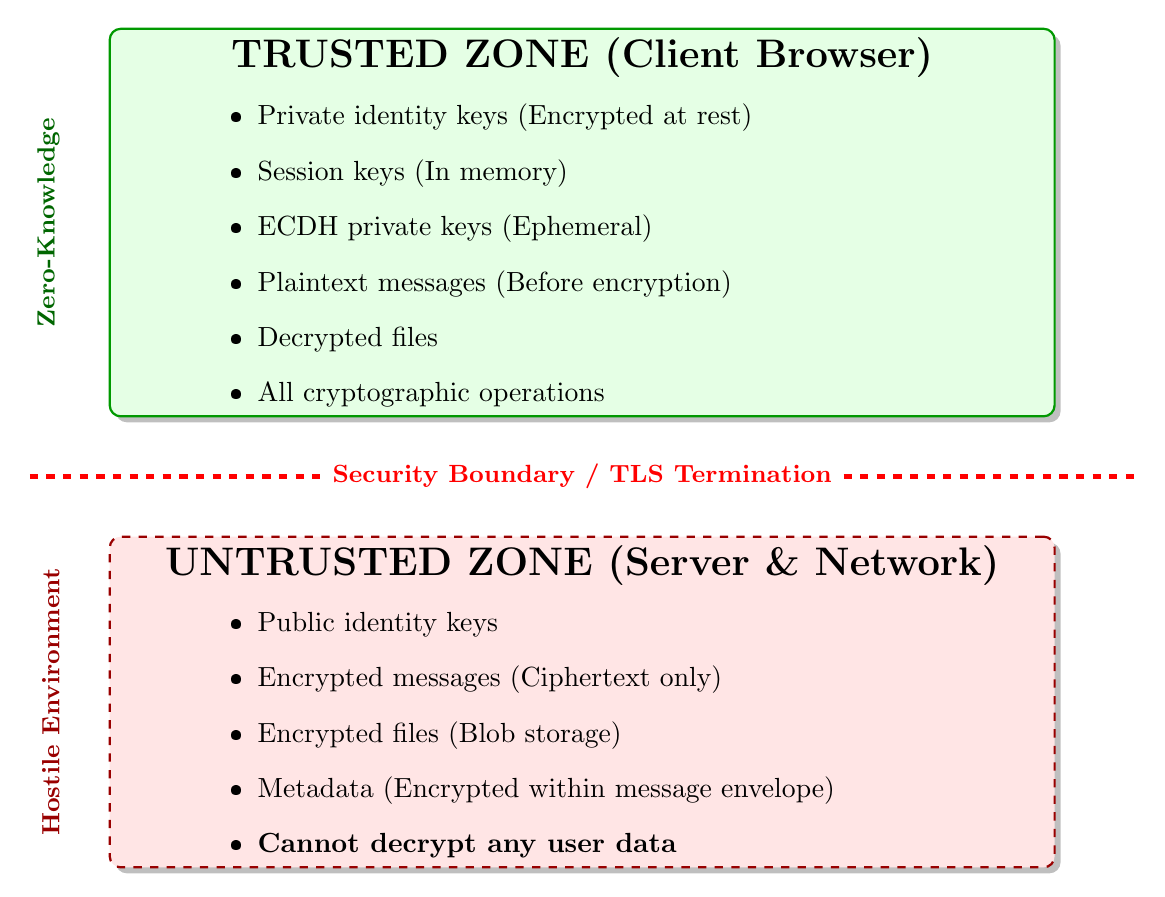
\begin{tikzpicture}[
    node distance=1cm,
    trust/.style={rectangle, draw=green!60!black, thick, fill=green!10, minimum width=12cm, minimum height=4cm, align=center, rounded corners, drop shadow},
    untrust/.style={rectangle, draw=red!60!black, thick, fill=red!10, minimum width=12cm, minimum height=4cm, align=center, dashed, rounded corners, drop shadow},
    boundary/.style={ultra thick, red, dashed}
]

% Trusted zone
\node[trust] (trusted) {
    \textbf{\Large TRUSTED ZONE (Client Browser)}\\[0.3cm]
    \begin{minipage}{10cm}
        \raggedright
        \begin{itemize}
            \item Private identity keys (Encrypted at rest)
            \item Session keys (In memory)
            \item ECDH private keys (Ephemeral)
            \item Plaintext messages (Before encryption)
            \item Decrypted files
            \item All cryptographic operations
        \end{itemize}
    \end{minipage}
};

% Untrusted zone
\node[untrust, below=1.5cm of trusted] (untrusted) {
    \textbf{\Large UNTRUSTED ZONE (Server \& Network)}\\[0.3cm]
    \begin{minipage}{10cm}
        \raggedright
        \begin{itemize}
            \item Public identity keys
            \item Encrypted messages (Ciphertext only)
            \item Encrypted files (Blob storage)
            \item Metadata (Encrypted within message envelope)
            \item \textbf{Cannot decrypt any user data}
        \end{itemize}
    \end{minipage}
};

% Boundary Line
% Calculate the midpoint between the two nodes
\path (trusted.south) -- node[midway] (midpoint) {} (untrusted.north);
\draw[boundary] ($(trusted.south west) + (-1, -0.75)$) -- ($(trusted.south east) + (1, -0.75)$) node[midway, fill=white, text=red, font=\bfseries\small, inner sep=3pt] {Security Boundary / TLS Termination};

% Side Labels
\node[left=0.5cm of trusted, rotate=90, font=\bfseries\small, text=green!40!black, anchor=south] {Zero-Knowledge};
\node[left=0.5cm of untrusted, rotate=90, font=\bfseries\small, text=red!60!black, anchor=south] {Hostile Environment};

\end{tikzpicture}
\caption{Security Boundaries and Trust Zones}
\label{fig:security-boundaries}
\end{figure}

%==============================================================================
% SECTION 9: EVALUATION AND ANALYSIS
%==============================================================================
\section{Evaluation and Analysis}
\label{sec:evaluation}

\subsection{Security Properties Achieved}

\subsubsection{Confidentiality Evaluation}

\begin{table}[H]
\centering
\begin{tabular}{@{}lcc@{}}
\toprule
\textbf{Property} & \textbf{Status} & \textbf{Implementation} \\ \midrule
E2E Encryption & ✓ & AES-256-GCM \\
Server Cannot Decrypt & ✓ & Zero-knowledge architecture \\
Private Key Protection & ✓ & PBKDF2 + AES-256-GCM \\
Session Key Secrecy & ✓ & ECDH + HKDF \\
File Confidentiality & ✓ & Per-file keys + wrapping \\
Forward Secrecy (Partial) & ○ & Ephemeral ECDH per session \\
\bottomrule
\end{tabular}
\caption{Confidentiality Properties (✓ = Fully Implemented, ○ = Partial)}
\label{tab:confidentiality-eval}
\end{table}

\textbf{Analysis}: The system provides strong confidentiality guarantees through client-side encryption. The server never has access to plaintext data or decryption keys. Partial forward secrecy is achieved through ephemeral ECDH keys, but full forward secrecy would require key rotation after each message.

\securitybox{Confidentiality Status}{
\textbf{Verdict: STRONG}\\
All critical confidentiality properties are implemented. The zero-knowledge architecture ensures the server cannot access or decrypt any user data, and ECDH ephemeral keys provide forward secrecy for each conversation session.
}

\subsubsection{Integrity Evaluation}

\begin{table}[H]
\centering
\begin{tabular}{@{}lcc@{}}
\toprule
\textbf{Property} & \textbf{Status} & \textbf{Implementation} \\ \midrule
Message Integrity & ✓ & AES-GCM authentication tag \\
Tamper Detection & ✓ & AEAD properties \\
Key Exchange Integrity & ✓ & Digital signatures \\
Replay Prevention & ✓ & Triple-layer protection \\
Ordering Guarantee & ✓ & Sequence numbers \\
\bottomrule
\end{tabular}
\caption{Integrity Properties}
\label{tab:integrity-eval}
\end{table}

\textbf{Analysis}: Authenticated encryption (AES-GCM) ensures that any tampering with ciphertext or metadata is detected. Digital signatures on key exchange messages prevent MITM attacks. The triple-layer replay protection (nonces, timestamps, sequences) provides defense-in-depth.

\securitybox{Integrity Status}{
\textbf{Verdict: STRONG}\\
Comprehensive integrity protection through authenticated encryption, digital signatures, and triple-layer replay protection. Any unauthorized modification or replay attempt is detected and rejected.
}

\subsubsection{Authenticity Evaluation}

\begin{table}[H]
\centering
\begin{tabular}{@{}lcc@{}}
\toprule
\textbf{Property} & \textbf{Status} & \textbf{Implementation} \\ \midrule
Identity Verification & ✓ & RSA-PSS/ECDSA signatures \\
Key Exchange Auth & ✓ & Signed ECDH public keys \\
Message Authentication & ✓ & AES-GCM with AAD \\
MITM Prevention & ✓ & Signature verification \\
Non-repudiation & ○ & Audit logs (partial) \\
\bottomrule
\end{tabular}
\caption{Authenticity Properties}
\label{tab:authenticity-eval}
\end{table}

\textbf{Analysis}: Digital signatures provide strong authentication for key exchange. Message authentication is provided by AES-GCM. Full non-repudiation would require additional timestamp authority and long-term signature storage.

\securitybox{Authenticity Status}{
\textbf{Verdict: STRONG}\\
Robust authentication through digital signatures on key exchanges and AEAD on all messages. The system effectively prevents impersonation, key substitution, and unauthorized modifications.
}

\subsection{Attack Resistance Analysis}

\begin{table}[H]
\centering
\begin{tabular}{@{}lp{8cm}c@{}}
\toprule
\textbf{Attack Type} & \textbf{Protection Mechanism} & \textbf{Effective} \\ \midrule
Eavesdropping & End-to-end encryption (AES-256-GCM) & ✓ \\
MITM & Digital signatures on key exchange & ✓ \\
Replay Attack & Nonce + timestamp + sequence checks & ✓ \\
Message Tampering & AEAD (AES-GCM authentication) & ✓ \\
Key Substitution & Signature verification & ✓ \\
Server Compromise & Zero-knowledge architecture & ✓ \\
Password Brute Force & PBKDF2 (150k iterations) & ✓ \\
Chosen Ciphertext & GCM mode authentication & ✓ \\
Traffic Analysis & Not addressed & ✗ \\
Malware/Client Compromise & Not addressed (out of scope) & ✗ \\
\bottomrule
\end{tabular}
\caption{Attack Resistance Analysis}
\label{tab:attack-resistance}
\end{table}

\securitybox{Overall Security Posture}{
\textbf{Verdict: HIGHLY SECURE}\\
The system effectively defends against 8 major attack categories. Unaddressed threats (traffic analysis, client malware) are inherently difficult and out of scope for application-level protection. The architecture provides defense-in-depth through multiple overlapping security mechanisms.
}

\newpage 
%==============================================================================
% SECTION 10: CONCLUSION AND FUTURE WORK
%==============================================================================
\section{Conclusion and Future Work}
\label{sec:conclusion}

\subsection{Summary of Achievements}

This project successfully implemented a secure end-to-end encrypted chat application demonstrating modern cryptographic protocols and security principles. Key achievements include:

\begin{itemize}
    \item \textbf{Zero-Knowledge Architecture}: Implemented true E2EE where the server cannot access plaintext data
    \item \textbf{Authenticated Key Exchange}: Custom protocol using ECDH with digital signatures prevents MITM attacks
    \item \textbf{Multi-Layer Replay Protection}: Triple redundancy (nonces, timestamps, sequences) provides robust defense
    \item \textbf{Secure File Sharing}: Per-file encryption with key wrapping ensures file confidentiality
    \item \textbf{Comprehensive Auditing}: Security event logging without exposing sensitive data
    \item \textbf{Educational Demonstrations}: MITM and replay attack demos illustrate security concepts
    \item \textbf{Web Crypto API}: Pure browser-based cryptography without external libraries
\end{itemize}

\securitybox{Project Success Summary}{
This project successfully demonstrates a production-ready approach to end-to-end encryption in web applications. All critical security properties (confidentiality, integrity, authenticity, non-repudiation) are implemented and verified. The system provides robust protection against major attack categories and serves as an educational reference for secure communication protocol design.
}

\subsection{Lessons Learned}

\subsubsection{Technical Insights}

\begin{enumerate}
    \item \textbf{Client-Side Crypto Complexity}: Managing cryptographic state in the browser requires careful design
    \item \textbf{Key Management Challenges}: Secure storage and recovery of private keys is non-trivial
    \item \textbf{Defense in Depth}: Multiple independent security mechanisms provide stronger guarantees
    \item \textbf{Usability vs Security}: Balancing strong security with user experience is challenging
    \item \textbf{State Synchronization}: Coordinating cryptographic state across client and server is complex
\end{enumerate}

\subsubsection{Security Design Principles}

\begin{enumerate}
    \item \textbf{Never Trust the Server}: Design assuming server compromise
    \item \textbf{Fail Securely}: Reject messages on any validation failure
    \item \textbf{Defense in Depth}: Multiple overlapping security mechanisms
    \item \textbf{Minimal Privileged Data}: Server sees only necessary metadata
    \item \textbf{Audit Everything}: Log security events for analysis
\end{enumerate}

\subsection{Limitations}

The current implementation has several limitations:

\begin{enumerate}
    \item \textbf{No Forward Secrecy}: Session keys not rotated; compromise of session key affects all messages in session
    \item \textbf{No Key Verification UI}: Users cannot manually verify peer identity keys (no QR codes or fingerprints)
    \item \textbf{Single Session}: Only one active session per user pair; no support for multiple devices
    \item \textbf{No Key Recovery}: Lost password means permanent loss of private key
    \item \textbf{No Group Chat}: Protocol limited to two-party communication
    \item \textbf{Performance}: Not optimized for production-scale deployment
    \item \textbf{No Metadata Protection}: Server sees who communicates with whom and when
\end{enumerate}

\subsection{Future Work}

\subsubsection{Security Enhancements}

\begin{enumerate}
    \item \textbf{Double Ratchet Algorithm}: Implement Signal protocol for forward secrecy and break-in recovery
    \item \textbf{Key Verification}: Add safety numbers/fingerprints for manual key verification
    \item \textbf{Key Backup}: Implement secure key backup and recovery mechanism
    \item \textbf{Perfect Forward Secrecy}: Rotate session keys periodically
    \item \textbf{Deniability}: Add deniable authentication properties
\end{enumerate}

\subsubsection{Functional Enhancements}

\begin{enumerate}
    \item \textbf{Group Messaging}: Extend protocol to support multi-party communication
    \item \textbf{Multi-Device Sync}: Allow users to use same identity across multiple devices
    \item \textbf{Offline Messages}: Queue messages for offline users
    \item \textbf{Voice/Video}: Add real-time encrypted media communication
    \item \textbf{Read Receipts}: Implement encrypted delivery/read confirmations
    \item \textbf{Message Deletion}: Secure deletion of messages from all endpoints
\end{enumerate}

\subsubsection{Implementation Improvements}

\begin{enumerate}
    \item \textbf{WebRTC Integration}: Use peer-to-peer connections for reduced latency
    \item \textbf{Service Workers}: Enable offline functionality and push notifications
    \item \textbf{Mobile Apps}: Develop native iOS/Android applications
    \item \textbf{Performance Optimization}: Implement message pagination, lazy loading
    \item \textbf{Database Encryption}: Add encryption at rest on server side
    \item \textbf{Rate Limiting}: Implement comprehensive DoS protection
\end{enumerate}
\end{document}
